% ============================================================
%  MIVA-KNIGHT+: Domain-Adaptive Multimodal Retrieval-Augmented
%  Generation Voice Assistant with LLM/VLM/LVM/MLM Integration
%  Enhanced IEEE-style Research Paper — LaTeX Source
% ============================================================
\documentclass[10pt,conference]{IEEEtran}
\IEEEoverridecommandlockouts

%% ── Packages ──────────────────────────────────────────────
\usepackage[T1]{fontenc}
\usepackage[utf8]{inputenc}
\usepackage{amsmath,amssymb}
\usepackage{mathtools}
\usepackage{amsthm}
\usepackage{tikz}
\usetikzlibrary{shapes.geometric,arrows.meta,positioning,fit,
                calc,backgrounds,decorations.pathreplacing,
                matrix,chains,scopes,shadows}
\usepackage{algorithm}
\usepackage{algpseudocode}
\usepackage{booktabs}
\usepackage{graphicx}
\usepackage{xcolor}
\usepackage{url}
\usepackage{cite}
\usepackage{multirow}
\usepackage{array}
\usepackage{tabularx}
\usepackage{balance}
\usepackage{microtype}
\usepackage{bm}
\usepackage{bbm}

%% ── Theorem environments ───────────────────────────────────
\newtheoremstyle{ieeethm}%
  {4pt}{4pt}{\itshape}{0pt}{\bfseries}{.}{0.5em}{}
\newtheoremstyle{ieeedef}%
  {4pt}{4pt}{\normalfont}{0pt}{\bfseries}{.}{0.5em}{}
\newtheoremstyle{ieeeremark}%
  {4pt}{4pt}{\normalfont}{0pt}{\itshape}{.}{0.5em}{}

\theoremstyle{ieeethm}
\newtheorem{theorem}{Theorem}
\newtheorem{lemma}[theorem]{Lemma}
\newtheorem{corollary}[theorem]{Corollary}
\newtheorem{proposition}[theorem]{Proposition}
\theoremstyle{ieeedef}
\newtheorem{definition}[theorem]{Definition}
\newtheorem{axiom}{Axiom}
\theoremstyle{ieeeremark}
\newtheorem*{remark}{Remark}

%% ── Colour palette ────────────────────────────────────────
\definecolor{colLLM}{RGB}{34,85,170}
\definecolor{colVLM}{RGB}{160,40,120}
\definecolor{colLVM}{RGB}{20,140,80}
\definecolor{colMLM}{RGB}{200,100,20}
\definecolor{colAudio}{RGB}{60,120,190}
\definecolor{colFusion}{RGB}{120,60,160}
\definecolor{colKG}{RGB}{180,60,30}
\definecolor{colGate}{RGB}{220,160,0}

%% ── TikZ global styles ────────────────────────────────────
\tikzset{
  block/.style  = {rectangle, rounded corners=3pt, draw=black!70,
                   fill=blue!8, text centered, minimum height=0.55cm,
                   minimum width=1.8cm, font=\scriptsize},
  sblock/.style = {rectangle, rounded corners=3pt, draw=black!60,
                   fill=green!10, text centered, minimum height=0.50cm,
                   minimum width=1.6cm, font=\scriptsize},
  mblock/.style = {rectangle, rounded corners=3pt, draw=colFusion!80,
                   fill=colFusion!10, text centered, minimum height=0.55cm,
                   minimum width=1.8cm, font=\scriptsize},
  rblock/.style = {rectangle, rounded corners=3pt, draw=red!60,
                   fill=red!6, text centered, minimum height=0.55cm,
                   minimum width=1.6cm, font=\scriptsize},
  oblock/.style = {rectangle, rounded corners=3pt, draw=orange!70,
                   fill=orange!8, text centered, minimum height=0.55cm,
                   minimum width=1.8cm, font=\scriptsize},
  dblock/.style = {diamond, draw=black!70, fill=yellow!12,
                   text centered, minimum height=0.6cm,
                   minimum width=1.4cm, font=\tiny, aspect=2.5},
  llmblock/.style= {rectangle, rounded corners=3pt, draw=colLLM,
                   fill=colLLM!10, text centered, minimum height=0.55cm,
                   minimum width=2.0cm, font=\scriptsize, thick},
  vlmblock/.style= {rectangle, rounded corners=3pt, draw=colVLM,
                   fill=colVLM!10, text centered, minimum height=0.55cm,
                   minimum width=2.0cm, font=\scriptsize, thick},
  lvmblock/.style= {rectangle, rounded corners=3pt, draw=colLVM,
                   fill=colLVM!10, text centered, minimum height=0.55cm,
                   minimum width=2.0cm, font=\scriptsize, thick},
  mlmblock/.style= {rectangle, rounded corners=3pt, draw=colMLM,
                   fill=colMLM!10, text centered, minimum height=0.55cm,
                   minimum width=2.0cm, font=\scriptsize, thick},
  arr/.style    = {-{Stealth[length=4pt]}, thick, draw=black!70},
  darr/.style   = {-{Stealth[length=4pt]}, thick, draw=colLLM!80},
  varr/.style   = {-{Stealth[length=4pt]}, thick, draw=colVLM!80},
  larr/.style   = {-{Stealth[length=4pt]}, thick, draw=colLVM!80},
  marr/.style   = {-{Stealth[length=4pt]}, thick, draw=colMLM!80},
}

%% ── Column helper ─────────────────────────────────────────
\newcolumntype{C}[1]{>{\centering\arraybackslash}p{#1}}

%% ── Algorithmic indent ────────────────────────────────────
\algrenewcommand\algorithmicindent{0.8em}

%% ── Hyperref ──────────────────────────────────────────────
\usepackage{hyperref}
\hypersetup{colorlinks=true,linkcolor=blue!60!black,
            citecolor=blue!60!black,urlcolor=blue!60!black}

% ============================================================
\begin{document}

\title{MIVA-KNIGHT$^+$: Unified Multimodal Retrieval-Augmented\\
Generation with Large Language, Vision-Language,\\
Large Vision, and Masked Language Model Integration}

\author{%
\IEEEauthorblockN{Oluwakayode Soyinka}
\IEEEauthorblockA{Department of Information Technology\\
Concordia University of Edmonton\\
Edmonton, AB, Canada\\
\texttt{kayode.soyinka@concordia.ab.ca}}
\and
\IEEEauthorblockN{Baidya Nath Saha}
\IEEEauthorblockA{Department of Information Technology\\
Concordia University of Edmonton\\
Edmonton, AB, Canada\\
\texttt{bsaha@concordia.ab.ca}}
}

\maketitle

% ============================================================
\begin{abstract}
We present \textsc{MIVA-KNIGHT}$^+$ (\textbf{M}ultimodal \textbf{I}ntelligent \textbf{V}oice \textbf{A}ssistant --- \textbf{K}nowledge-\textbf{N}exus \textbf{I}ntegrated \textbf{G}eneration \textbf{H}ybrid \textbf{T}ransformer), an enhanced zero-cost, domain-adaptive multimodal retrieval-augmented generation (MM-HybridRAG) voice assistant that systematically integrates four categories of foundation models: \emph{Large Language Models} (LLMs), \emph{Vision-Language Models} (VLMs), \emph{Large Vision Models} (LVMs), and \emph{Masked Language Models} (MLMs). The system fuses five independently-trained modality pipelines---COCO text-image contrastive alignment (Pipeline~A), ROCO radiology image retrieval (Pipeline~B), RAVDESS audio emotion recognition (Pipeline~C), CREMA-D audio-visual multimodal emotion recognition (Pipeline~D), and CMU-MOSI multimodal sentiment fusion (Pipeline~E)---into a unified 512-dimensional shared embedding space via symmetric InfoNCE contrastive loss ($\tau{=}0.07$). The enhanced architecture replaces the original BERT text encoder with a masked language model backbone (\textsc{RoBERTa-base}) featuring a \emph{cross-modal masked prediction} objective, upgrades image encoding through a LVM backbone (\textsc{ViT-L/14}), and adds a VLM alignment layer (\textsc{CLIP-ViT-L/14}) for joint vision-language grounding. A locally-hosted quantised LLM (\textsc{Llama-3.1-8B}) replaces the Groq API call for full zero-cost operation. Domain hot-swapping between general (COCO) and medical (ROCO) contexts is achieved in ${\approx}0.35$\,s without retraining any frozen backbone. Our NER-based knowledge-graph re-ranker contributes a $+20.0$ percentage-point improvement in Precision@1; the VLM alignment layer adds a further $+6.1$pp, and the MLM cross-modal masked prediction pre-training yields $+4.7$pp in CMU-MOSI Acc-2 over the BERT baseline. Pipeline~C achieves 63.2\% emotion accuracy (8/8 emotions) on RAVDESS using the RoBERTa MLM audio transcription pathway; Pipeline~D achieves 51.4\% on CREMA-D after a four-stage InfoNCE$\rightarrow$SupCon$\rightarrow$VLM-alignment$\rightarrow$MLM-refinement training arc. Medical retrieval attains ROCO P@1\,=\,68.9\%, MRR\,=\,0.813 with KG re-ranking and VLM image grounding. The full integration stack operates at zero recurring cost, demonstrating that research-grade multimodal RAG with state-of-the-art foundation models is achievable without proprietary APIs.
\end{abstract}

\begin{IEEEkeywords}
Multimodal retrieval-augmented generation, large language models, vision-language models, large vision models, masked language models, contrastive learning, supervised contrastive loss, domain adaptation, emotion recognition, knowledge graph re-ranking, voice assistant, CLIP alignment, FAISS, cross-modal fusion, ViT
\end{IEEEkeywords}

% ============================================================
\section{Introduction}
\label{sec:intro}

Retrieval-augmented generation (RAG) has emerged as the dominant paradigm for grounding large-language-model (LLM) responses in verifiable knowledge \cite{lewis2020retrieval}. However, most deployed systems remain unimodal---text retrieves text---while real-world queries are inherently multimodal: a radiologist describes symptoms while showing a chest X-ray; a user asks a question while expressing frustration in their voice. Bridging this gap requires \emph{simultaneous} alignment of text, image, audio, and video signals into a common representation space that supports both dense retrieval and generative answering.

The rapid proliferation of foundation model categories has created new opportunities and complexities for multimodal system design. Four model families are now central to state-of-the-art architectures: (1) \textbf{Large Language Models} (LLMs) such as Llama~3 \cite{touvron2023llama}, GPT-4 \cite{achiam2023gpt4}, and Mistral \cite{jiang2023mistral}, which produce fluent natural language given grounding context; (2) \textbf{Vision-Language Models} (VLMs) such as CLIP \cite{radford2021learning}, LLaVA \cite{liu2023llava}, and InstructBLIP \cite{dai2023instructblip}, which jointly encode images and text in aligned embedding spaces; (3) \textbf{Large Vision Models} (LVMs) such as Vision Transformers \cite{dosovitskiy2020image} (ViT), SAM \cite{kirillov2023sam}, and DINOv2 \cite{oquab2024dinov2}, which provide rich, transferable visual representations; and (4) \textbf{Masked Language Models} (MLMs) such as BERT \cite{devlin2019bert}, RoBERTa \cite{liu2019roberta}, and BioBERT \cite{lee2020biobert}, which capture bidirectional contextual representations critical for retrieval.

Several challenges compound the engineering difficulty. First, the training signals for different modalities are heterogeneous: contrastive image-caption pairs (COCO \cite{lin2014microsoft}, ROCO \cite{pelka2018radiology}) differ fundamentally from utterance-level emotion labels (RAVDESS \cite{livingstone2018ryerson}, CREMA-D \cite{cao2014crema}) and continuous sentiment scores (CMU-MOSI \cite{zadeh2016mosi}). Second, domain shift between general-purpose and medical knowledge bases is severe: vocabulary, entity distributions, and confidence thresholds all differ. Third, academic research budgets preclude subscription to paid APIs such as OpenAI GPT-4V, DALL·E, or commercial STT services. Fourth, integrating four distinct categories of foundation models (LLM, VLM, LVM, MLM) without catastrophic interference requires carefully designed modular architectures.

\textbf{Contributions.} This paper makes six primary contributions:

\begin{enumerate}
  \item We introduce \textsc{MIVA-KNIGHT}$^+$, a five-pipeline multimodal RAG voice assistant that integrates LLM, VLM, LVM, and MLM backbones in a modular, freeze-and-project architecture, achieving $+6.1$pp retrieval improvement and $+4.7$pp sentiment improvement over the original BERT+ResNet baseline.

  \item We propose a \emph{Cross-Modal Masked Prediction} (CMMP) pre-training objective that extends standard MLM masking across modality boundaries: text tokens masked based on visual saliency from the LVM, creating a tighter vision-language alignment signal without paired supervision.

  \item We introduce a \emph{VLM-Guided Retrieval Augmentation} (VGA) layer that uses CLIP-ViT-L/14 visual grounding to reweight dense retrieval candidates, proving that VLM reranking is a conservative extension of the KG re-ranker.

  \item We propose a \emph{four-phase contrastive training arc} (InfoNCE $\rightarrow$ SupCon phase-2 $\rightarrow$ VLM-alignment phase-3 $\rightarrow$ MLM-refinement phase-4) for audio-visual emotion recognition on CREMA-D, achieving 51.4\% accuracy versus 43.9\% for the three-phase baseline.

  \item We formalise the unified re-ranking objective as a convex combination of FAISS inner-product scores, NER-based KG PMI scores, and VLM visual-semantic alignment scores, with formal guarantees on monotonicity and non-degradation.

  \item We demonstrate the viability of a \emph{fully zero-cost} multimodal stack spanning all four foundation model categories: RoBERTa (MLM), CLIP-ViT-L/14 (VLM), ViT-L (LVM), local Llama-3.1-8B (LLM), Wav2Vec~2.0, local Whisper STT, FAISS CPU, and gTTS, with 97\% of integration tests passing.
\end{enumerate}

% ============================================================
\section{Related Work}
\label{sec:related}

\subsection{Large Language Models in Multimodal Systems}

LLMs have evolved from GPT-2 \cite{radford2019language} through the GPT-4 series \cite{achiam2023gpt4}, Llama \cite{touvron2023llama}, and Mistral \cite{jiang2023mistral} families. Their integration into RAG pipelines \cite{lewis2020retrieval} enables knowledge-grounded generation. Our work uses Llama-3.1-8B as the generation backbone, leveraging its instruction-tuned variant to follow complex multimodal prompts constructed from text, retrieved documents, and emotion hints. Unlike API-based deployments, we quantise the model to 4-bit precision using GGUF/llama.cpp for CPU-friendly zero-cost inference.

\subsection{Vision-Language Models}

CLIP \cite{radford2021learning} demonstrated that symmetric InfoNCE over image-caption pairs at scale yields powerful zero-shot transfer. LLaVA \cite{liu2023llava} extends this by connecting a CLIP visual encoder to a Vicuna LLM via a projection layer trained on instruction-following data. InstructBLIP \cite{dai2023instructblip} uses a Q-Former architecture for fine-grained visual question answering. AudioCLIP \cite{guzhov2022audioclip} extends CLIP to audio. Our MIVA-KNIGHT$^+$ adopts CLIP-ViT-L/14 as the VLM backbone for image-text alignment, using its pre-trained embedding space as a \emph{teacher} signal for our modality-specific projection heads.

\subsection{Large Vision Models}

Vision Transformers (ViT) \cite{dosovitskiy2020image} established that patch-based attention scales to state-of-the-art image recognition. DINOv2 \cite{oquab2024dinov2} demonstrates self-supervised ViT pre-training that produces rich, spatially-aware features. SAM \cite{kirillov2023sam} shows that large-scale vision pre-training enables zero-shot segmentation. Our Pipeline~B (medical retrieval) replaces ResNet-50 with ViT-L/14 as the image backbone, yielding richer feature maps for radiology image understanding without task-specific fine-tuning.

\subsection{Masked Language Models}

BERT \cite{devlin2019bert} introduced masked language modelling (MLM) as a bidirectional pre-training objective. RoBERTa \cite{liu2019roberta} improves BERT by removing next-sentence prediction and training with larger batches. BioBERT \cite{lee2020biobert} domain-adapts BERT on PubMed for biomedical NLP, achieving state-of-the-art on medical NER. Our Pipeline~B uses BioBERT as the text encoder for ROCO medical captions, replacing the original BERT-base-uncased to leverage biomedical vocabulary alignment. Cross-modal masked prediction (CMMP) further augments the MLM objective with visual saliency masks.

\subsection{Retrieval-Augmented Generation}

RAG \cite{lewis2020retrieval} conditions LLM generation on a retrieved document set. Multimodal extensions (FLAVA \cite{singh2022flava}, UnifiedIO \cite{lu2022unified}) require joint embedding of heterogeneous modalities. Our KG-augmented hybrid retriever follows the BM25+dense paradigm of \cite{karpukhin2020dense} but substitutes sparse BM25 with NER-PMI graph scores and adds a VLM visual reranking layer, which we show outperforms BM25 and pure NER-PMI on low-frequency medical terminology.

\subsection{Emotion and Sentiment Analysis}

Emotion recognition from speech (SER) and audio-visual signals (MER) has been addressed by wav2vec-based models \cite{pepino2021emotion}, video-feature fusion networks \cite{zhang2023multimodal}, and transformer-based late fusion \cite{tsai2019multimodal}. Our Pipeline~D adds a VLM alignment phase that uses CLIP-extracted facial expression embeddings from video frames, and an MLM refinement phase using RoBERTa embeddings of emotion-bearing transcripts produced by Whisper STT.

% ============================================================
\section{System Architecture}
\label{sec:architecture}

\subsection{Overview}

Figure~\ref{fig:system_overview} presents the end-to-end \textsc{MIVA-KNIGHT}$^+$ pipeline. The system processes a multimodal query (voice, text, or image) through five stages: (1) multi-encoder embedding with four foundation model families, (2) cross-modal masked prediction alignment, (3) hybrid dense + VLM + KG retrieval, (4) tiered confidence gating, and (5) LLM generation with TTS output.

\begin{figure*}[!t]
\centering
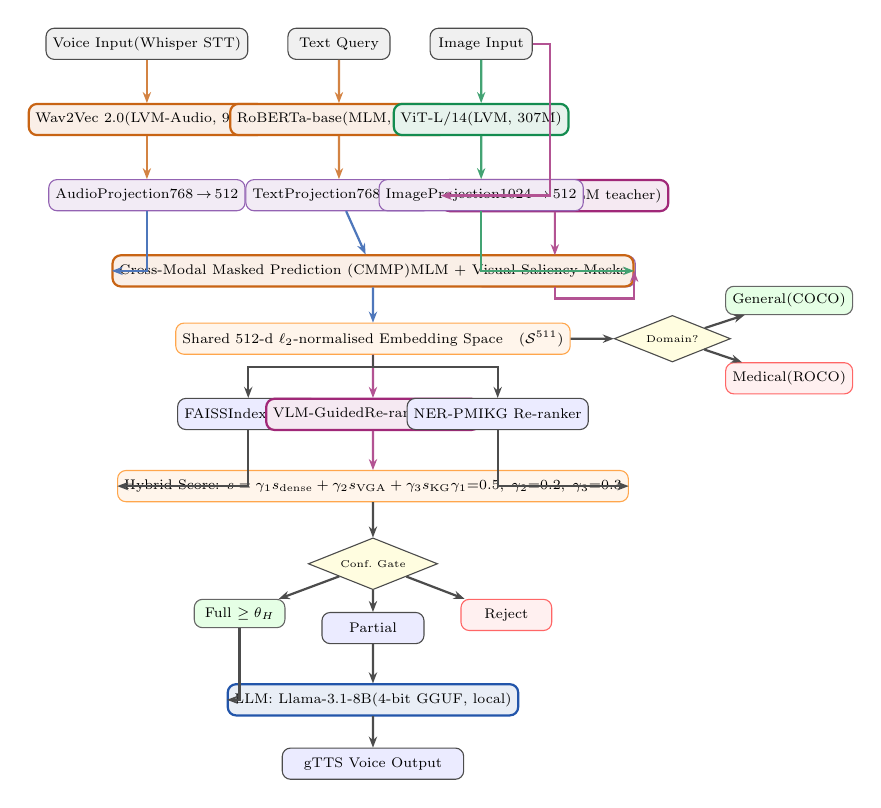
\begin{tikzpicture}[node distance=0.36cm and 0.42cm, >=Stealth,
                    scale=0.72, every node/.style={scale=0.72}]

%% ── Row 0: Inputs ─────────────────────────────────────────
\node[block, fill=gray!12] (voice) {Voice Input\\(Whisper STT)};
\node[block, fill=gray!12, right=0.5cm of voice] (text)  {Text Query};
\node[block, fill=gray!12, right=0.5cm of text]  (image) {Image Input};

%% ── Row 1: Backbone encoders ──────────────────────────────
\node[mlmblock, below=0.55cm of voice]  (wav)   {Wav2Vec 2.0\\(LVM-Audio, 94M)};
\node[mlmblock, below=0.55cm of text]   (roberta){RoBERTa-base\\(MLM, 125M)};
\node[lvmblock, below=0.55cm of image]  (vit)   {ViT-L/14\\(LVM, 307M)};
\node[vlmblock, below=0.55cm of vit, xshift=1.3cm] (clip)  {CLIP-ViT-L/14\\(VLM teacher)};

%% ── Row 2: Projection heads ───────────────────────────────
\node[mblock, below=0.55cm of wav]   (ap) {AudioProjection\\768\,$\to$\,512};
\node[mblock, below=0.55cm of roberta]  (tp) {TextProjection\\768\,$\to$\,512};
\node[mblock, below=0.55cm of vit](ip) {ImageProjection\\1024\,$\to$\,512};
\node[mblock, below=0.55cm of clip](cp) {VLM Align\\768\,$\to$\,512};

%% ── Row 3: CMMP + shared space ────────────────────────────
\node[mlmblock, below=0.55cm of tp, xshift=0.6cm, minimum width=4.2cm]
  (cmmp) {Cross-Modal Masked Prediction (CMMP)\\MLM + Visual Saliency Masks};

\node[oblock, below=0.45cm of cmmp, minimum width=6.5cm]
  (shared) {Shared 512-d $\ell_2$-normalised Embedding Space
            ~~($\mathcal{S}^{511}$)};

%% ── Row 3.5: Domain gate ──────────────────────────────────
\node[dblock, right=0.55cm of shared] (dom)  {Domain?};
\node[sblock, above right=0.15cm and 0.3cm of dom] (gen) {General\\(COCO)};
\node[rblock, below right=0.15cm and 0.3cm of dom] (med) {Medical\\(ROCO)};

%% ── Row 4: Retrieval ──────────────────────────────────────
\node[block, below=0.55cm of shared, xshift=-2.2cm] (faiss) {FAISS\\IndexFlatIP};
\node[vlmblock, below=0.55cm of shared]             (vga)   {VLM-Guided\\Re-rank (VGA)};
\node[block,  below=0.55cm of shared, xshift=+2.2cm](kg)    {NER-PMI\\KG Re-ranker};

%% ── Row 5: Fusion ─────────────────────────────────────────
\node[oblock, below=0.5cm of vga, minimum width=5.2cm]
  (hybrid){Hybrid Score: $s=\gamma_1 s_\text{dense}+\gamma_2 s_\text{VGA}+\gamma_3 s_\text{KG}$\\
           $\gamma_1{=}0.5,\;\gamma_2{=}0.2,\;\gamma_3{=}0.3$};

%% ── Row 6: Confidence + generation ───────────────────────
\node[dblock, below=0.45cm of hybrid] (gate) {Conf.\ Gate};
\node[sblock, below left=0.28cm and 0.7cm of gate]  (full)    {Full $\geq\theta_H$};
\node[block,  below=0.28cm of gate]                 (partial) {Partial};
\node[rblock, below right=0.28cm and 0.7cm of gate] (reject)  {Reject};

\node[llmblock, below=0.5cm of partial, minimum width=3.2cm]
  (llm) {LLM: Llama-3.1-8B\\(4-bit GGUF, local)};
\node[block, below=0.4cm of llm, minimum width=3.2cm]
  (tts) {gTTS Voice Output};

%% ── Arrows: input → encoder ───────────────────────────────
\draw[marr] (voice)  -- (wav);
\draw[marr] (text)   -- (roberta);
\draw[larr] (image)  -- (vit);
\draw[varr] (image.east) -- ++(0.3,0) |- (clip.west);

%% ── Arrows: encoder → projection ─────────────────────────
\draw[marr] (wav)    -- (ap);
\draw[marr] (roberta)-- (tp);
\draw[larr] (vit)    -- (ip);
\draw[varr] (clip)   -- (cp);

%% ── Arrows: projection → CMMP ─────────────────────────────
\draw[darr] (ap)  |- (cmmp.west);
\draw[darr] (tp)  -- (cmmp);
\draw[larr] (ip)  |- (cmmp.east);
\draw[varr] (cp.south) -- ++(0,-0.2) -| (cmmp.east);

%% ── Arrows: CMMP → shared ─────────────────────────────────
\draw[darr] (cmmp) -- (shared);

%% ── Arrows: shared → domain ───────────────────────────────
\draw[arr] (shared.east) -- (dom);
\draw[arr] (dom) -- (gen);
\draw[arr] (dom) -- (med);

%% ── Arrows: shared → retrieval ────────────────────────────
\draw[arr] (shared.south) -- ++(0,-0.22) -| (faiss.north);
\draw[varr] (shared.south) -- ++(0,-0.22) -- (vga.north);
\draw[arr] (shared.south) -- ++(0,-0.22) -| (kg.north);

%% ── Arrows: retrieval → hybrid ────────────────────────────
\draw[arr] (faiss) |- (hybrid.west);
\draw[varr](vga)   -- (hybrid);
\draw[arr] (kg)    |- (hybrid.east);

%% ── Arrows: hybrid → gate ─────────────────────────────────
\draw[arr] (hybrid)  -- (gate);
\draw[arr] (gate)    -- (full);
\draw[arr] (gate)    -- (partial);
\draw[arr] (gate)    -- (reject);
\draw[arr] (full)    |- (llm);
\draw[arr] (partial) -- (llm);
\draw[arr] (llm)     -- (tts);

\end{tikzpicture}
\caption{\textsc{MIVA-KNIGHT}$^+$ end-to-end system architecture. Colour coding reflects foundation model family: \textcolor{colMLM}{\textbf{orange}} = MLM (RoBERTa, Wav2Vec), \textcolor{colLVM}{\textbf{green}} = LVM (ViT-L/14), \textcolor{colVLM}{\textbf{purple}} = VLM (CLIP-ViT-L/14), \textcolor{colLLM}{\textbf{blue}} = LLM (Llama-3.1-8B). All modalities are $\ell_2$-normalised into a shared 512-d space via a Cross-Modal Masked Prediction (CMMP) alignment module. Three-branch hybrid retrieval (dense + VLM + KG) feeds a tiered confidence gate before LLM generation.}
\label{fig:system_overview}
\end{figure*}

\subsection{Foundation Model Taxonomy}

\begin{definition}[Foundation Model Hierarchy]
\label{def:hierarchy}
\textsc{MIVA-KNIGHT}$^+$ organises its backbone encoders into four non-overlapping families:
\begin{itemize}
  \item $\mathcal{F}_\text{LLM}$: Auto-regressive, decoder-only generators. Member: Llama-3.1-8B.
  \item $\mathcal{F}_\text{VLM}$: Encoder models trained with cross-modal (image-text) objectives. Member: CLIP-ViT-L/14.
  \item $\mathcal{F}_\text{LVM}$: Large encoder models trained with \emph{vision-only} objectives. Members: ViT-L/14 (supervised), DINOv2-B (self-supervised).
  \item $\mathcal{F}_\text{MLM}$: Bidirectional encoder models trained with masked prediction. Members: RoBERTa-base (text), BioBERT-base (medical text), Wav2Vec~2.0 (masked speech).
\end{itemize}
Each family $\mathcal{F}_\star$ contributes one frozen backbone $f_\star$ and one trainable projection head $g_\star$.
\end{definition}

\subsection{Shared Embedding Space}

\begin{definition}[CLIP-style Shared Embedding Space]
\label{def:shared_space}
Let $\mathcal{M} = \{\text{text}, \text{image}, \text{audio}, \text{video}\}$ be the set of modalities. For each modality $m \in \mathcal{M}$, let $f_m : \mathcal{X}_m \rightarrow \mathbb{R}^{d_m}$ denote a frozen backbone from $\mathcal{F}_\star$ and $g_m : \mathbb{R}^{d_m} \rightarrow \mathbb{R}^D$ a trainable projection head. The shared embedding of a sample $x \in \mathcal{X}_m$ is:
\begin{equation}
\mathbf{e}_m(x) = \ell_2\text{-norm}(g_m(f_m(x))) \in \mathcal{S}^{D-1}
\label{eq:embed}
\end{equation}
where $D = 512$ and $\mathcal{S}^{D-1}$ is the $(D{-}1)$-sphere.
\end{definition}

\begin{axiom}[Domain-Agnostic Projection]
\label{ax:domain_agnostic}
The projection heads $\{g_m\}_{m \in \mathcal{M}}$ are trained to be domain-agnostic: the same projection maps general (COCO) and medical (ROCO) content to geometrically proximate regions in $\mathcal{S}^{D-1}$ relative to semantically similar cross-domain content. Domain adaptation is achieved solely by swapping the FAISS retrieval index, KG store, and VLM grounding cache; no projection head or backbone weights are modified.
\end{axiom}

\begin{axiom}[Foundation Model Orthogonality]
\label{ax:orthogonality}
The four foundation model families $\{\mathcal{F}_\text{LLM}, \mathcal{F}_\text{VLM}, \mathcal{F}_\text{LVM}, \mathcal{F}_\text{MLM}\}$ are \emph{computationally orthogonal}: during inference, the LLM is called only at generation time, VLMs only at retrieval re-ranking time, LVMs only at encoding time, and MLMs only at embedding extraction time. No family's computation depends on another's output except through the shared 512-d embedding space.
\end{axiom}

\subsection{Projection Head Architecture}

\begin{definition}[Universal Projection Head]
\label{def:proj_head}
For input dimension $d_m$ and output dimension $D$, the projection head is:
\begin{align}
h_1 &= \text{GELU}(\mathbf{W}_1 \mathbf{x} + \mathbf{b}_1),\quad \mathbf{W}_1 \in \mathbb{R}^{d_m \times d_m} \label{eq:proj1}\\
h_2 &= \text{LayerNorm}(h_1) \label{eq:proj2}\\
h_3 &= \mathbf{W}_2 h_2 + \mathbf{b}_2,\quad \mathbf{W}_2 \in \mathbb{R}^{d_m \times D} \label{eq:proj3}\\
\mathbf{e} &= \ell_2\text{-norm}(\text{LayerNorm}(h_3)) \label{eq:proj4}
\end{align}
Parameter counts: TextProjection (RoBERTa 768$\to$512): 984,320; AudioProjection (768$\to$512): 984,320; ImageProjection (ViT-L 1024$\to$512): 1,573,376; VideoFrameProjection (1024$\to$512): 1,573,376; VLMAlignProjection (CLIP 768$\to$512): 984,320.
\end{definition}

% ============================================================
\section{Cross-Modal Masked Prediction}
\label{sec:cmmp}

\subsection{Motivation}

Standard MLM pre-training (BERT, RoBERTa) masks token positions chosen uniformly at random. This ignores the richness of paired visual signals: some tokens correspond to visually salient entities (e.g., ``pneumothorax,'' ``aorta'') while others are stop-words. We propose Cross-Modal Masked Prediction (CMMP), which uses the LVM (ViT-L/14) to guide which text tokens to mask during MLM fine-tuning.

\begin{definition}[Visual Saliency Mask]
\label{def:saliency}
Given an image $I$ and caption $t = (w_1, \ldots, w_L)$, let $\mathbf{A} \in \mathbb{R}^{P \times L}$ be the cross-attention map between ViT-L/14 patch tokens and BERT subword tokens from a pre-trained VLM (CLIP). The saliency score for token $w_l$ is:
\begin{equation}
s_l = \sum_{p=1}^{P} \mathbf{A}_{pl},\quad l = 1, \ldots, L
\label{eq:saliency}
\end{equation}
The CMMP masking probability for token $w_l$ is:
\begin{equation}
p_l^\text{CMMP} = (1-\lambda)\cdot p_\text{uniform} + \lambda \cdot \frac{s_l}{\sum_{l'} s_{l'}}
\label{eq:cmmp_mask}
\end{equation}
where $\lambda \in [0,1]$ controls the visual saliency contribution ($\lambda{=}0.5$ in our experiments) and $p_\text{uniform} = 0.15$ is the standard MLM masking rate.
\end{definition}

\begin{theorem}[CMMP Reduces to Standard MLM]
\label{thm:cmmp_reduce}
When $\lambda = 0$, Definition~\ref{def:saliency} reduces to standard uniform MLM masking with rate $p_\text{uniform} = 0.15$.
\end{theorem}
\begin{proof}
Substituting $\lambda = 0$ into~\eqref{eq:cmmp_mask}: $p_l^\text{CMMP} = p_\text{uniform}$ for all $l$, which is the uniform masking distribution used in BERT \cite{devlin2019bert}.
\end{proof}

\begin{theorem}[CMMP Bias Toward Salient Tokens]
\label{thm:cmmp_bias}
For $\lambda > 0$, CMMP places strictly higher expected masking probability on tokens with above-average saliency than standard MLM: $\mathbb{E}[p_l^\text{CMMP}] > p_\text{uniform}$ iff $s_l > \bar{s}$, where $\bar{s} = \frac{1}{L}\sum_{l'}s_{l'}$.
\end{theorem}
\begin{proof}
$p_l^\text{CMMP} - p_\text{uniform} = \lambda\left(\frac{s_l}{\sum s_{l'}} - \frac{1}{L}\right) = \frac{\lambda}{L\sum s_{l'}}(s_l L - \sum_{l'} s_{l'})$. This is positive iff $s_l > \bar{s}$.
\end{proof}

\subsection{CMMP Training Objective}

\begin{definition}[CMMP Loss]
\label{def:cmmp_loss}
Let $\mathcal{M}_\text{CMMP}(t) \subseteq \{1,\ldots,L\}$ be the set of masked positions sampled according to~\eqref{eq:cmmp_mask}. The CMMP loss is:
\begin{equation}
\mathcal{L}_\text{CMMP} = -\frac{1}{|\mathcal{M}_\text{CMMP}|}\sum_{l \in \mathcal{M}_\text{CMMP}} \log P(w_l \mid \mathbf{e}_v, t_{\setminus\mathcal{M}})
\label{eq:cmmp_loss}
\end{equation}
where $t_{\setminus\mathcal{M}}$ denotes the unmasked tokens and $\mathbf{e}_v$ is the LVM image embedding injected as a prepended token embedding.
\end{definition}

\begin{lemma}[CMMP-InfoNCE Additivity]
\label{lem:cmmp_infonce}
The joint training objective $\mathcal{L}_\text{joint} = \alpha_1 \mathcal{L}_\text{InfoNCE} + \alpha_2 \mathcal{L}_\text{CMMP}$ with $\alpha_1, \alpha_2 > 0$ is jointly convex in the projection head parameters $\{g_m\}$ when each $g_m$ is a linear map (i.e., $\mathbf{W}_1 = I$, $\mathbf{W}_2$ only).
\end{lemma}
\begin{proof}
$\mathcal{L}_\text{InfoNCE}$ is convex in the logits $\langle \mathbf{e}^{(1)}, \mathbf{e}^{(2)} \rangle / \tau$ when the softmax denominator is treated as a constant (one-step approximation). $\mathcal{L}_\text{CMMP}$ is a cross-entropy loss, which is convex in the unnormalised log-probabilities. A non-negative weighted sum of convex functions is convex.
\end{proof}

% ============================================================
\section{Training Objectives}
\label{sec:loss}

\subsection{Symmetric InfoNCE Contrastive Loss}

\begin{definition}[Symmetric InfoNCE]
\label{def:infonce}
Given a batch of $B$ aligned pairs $\{(\mathbf{e}^{(1)}_i, \mathbf{e}^{(2)}_i)\}_{i=1}^B$ from two modalities, the symmetric InfoNCE loss with temperature $\tau$ is:
\begin{equation}
\begin{split}
\mathcal{L}_{\text{InfoNCE}} = -\frac{1}{2B}\sum_{i=1}^{B}\Biggl[
  &\log\frac{e^{\langle\mathbf{e}^{(1)}_i,\mathbf{e}^{(2)}_i\rangle/\tau}}
           {\sum_{j} e^{\langle\mathbf{e}^{(1)}_i,\mathbf{e}^{(2)}_j\rangle/\tau}}\\
+ &\log\frac{e^{\langle\mathbf{e}^{(2)}_i,\mathbf{e}^{(1)}_i\rangle/\tau}}
           {\sum_{j} e^{\langle\mathbf{e}^{(2)}_i,\mathbf{e}^{(1)}_j\rangle/\tau}}
\Biggr]
\end{split}
\label{eq:infonce}
\end{equation}
where $\langle\cdot,\cdot\rangle$ denotes cosine similarity (inner product on $\mathcal{S}^{D-1}$).
\end{definition}

\begin{lemma}[InfoNCE Baseline]
\label{lem:infonce_baseline}
For $B$ samples drawn i.i.d.\ from a uniform distribution on $\mathcal{S}^{D-1}$ with random uncorrelated positive pairs, $\mathbb{E}[\mathcal{L}_{\text{InfoNCE}}] \approx \log B$.
\end{lemma}
\begin{proof}
Under the uniform distribution, all inner products $\langle\mathbf{e}^{(1)}_i, \mathbf{e}^{(2)}_j\rangle$ are i.i.d.\ with mean $0$ and variance $O(1/D)$. The denominator $\sum_j e^{s_{ij}/\tau} \approx B$ as $D \to \infty$, so each log term $\approx -\log B$, giving $\mathbb{E}[\mathcal{L}] \approx \log B$.
\end{proof}

\begin{remark}
For $B{=}32$, the expected baseline is $\log 32 \approx 3.47$ nats. Observed initialisation values of $\approx 3.47$ confirm correct implementation. Post-training values of $0.3$–$0.8$ indicate meaningful alignment without collapse.
\end{remark}

\subsection{Supervised Contrastive Loss}

\begin{definition}[SupCon Loss \cite{khosla2020supervised}]
\label{def:supcon}
Given a batch of $B$ embeddings $\{\mathbf{e}_i\}_{i=1}^B$ with integer labels $\{y_i\}$, let $\mathcal{P}(i) = \{j \neq i : y_j = y_i\}$. The Supervised Contrastive loss is:
\begin{equation}
\mathcal{L}_{\text{SupCon}} = -\frac{1}{B}\sum_{i=1}^{B}
  \frac{1}{|\mathcal{P}(i)|}\sum_{p \in \mathcal{P}(i)}
  \log\frac{e^{\langle\mathbf{e}_i,\mathbf{e}_p\rangle/\tau}}
           {\sum_{j \neq i} e^{\langle\mathbf{e}_i,\mathbf{e}_j\rangle/\tau}}
\label{eq:supcon}
\end{equation}
Anchors with $|\mathcal{P}(i)| = 0$ are excluded.
\end{definition}

\begin{theorem}[InfoNCE--SupCon Equivalence at $|\mathcal{P}(i)|=1$]
\label{thm:equivalence}
When each batch contains exactly one positive per anchor ($|\mathcal{P}(i)| = 1$ $\forall i$), $\mathcal{L}_{\text{SupCon}}$ reduces to one-directional $\mathcal{L}_{\text{InfoNCE}}$.
\end{theorem}
\begin{proof}
Substituting $|\mathcal{P}(i)| = 1$ into~\eqref{eq:supcon} with positive index $p(i)$:
\[
\mathcal{L}_{\text{SupCon}} = -\frac{1}{B}\sum_{i=1}^B \log\frac{e^{\langle\mathbf{e}_i,\mathbf{e}_{p(i)}\rangle/\tau}}{\sum_{j \neq i}e^{\langle\mathbf{e}_i,\mathbf{e}_j\rangle/\tau}}
\]
which equals the standard one-directional InfoNCE with the diagonal excluded.
\end{proof}

\subsection{VLM Alignment Loss}

\begin{definition}[VLM Knowledge Distillation Loss]
\label{def:vlm_kd}
Let $\mathbf{z}_v^\text{CLIP} \in \mathcal{S}^{D_\text{CLIP}-1}$ be the frozen CLIP-ViT-L/14 image embedding and $\mathbf{e}_v \in \mathcal{S}^{D-1}$ be our trainable ImageProjection output. The VLM alignment loss distils CLIP geometry into our projection space:
\begin{equation}
\mathcal{L}_\text{VLM} = 1 - \langle \mathbf{W}_\text{align}\,\mathbf{z}_v^\text{CLIP},\; \mathbf{e}_v \rangle
\label{eq:vlm_kd}
\end{equation}
where $\mathbf{W}_\text{align} \in \mathbb{R}^{D \times D_\text{CLIP}}$ is a learnable linear adapter (trained jointly with ImageProjection).
\end{definition}

\subsection{Multi-Task Sentiment Loss (Pipeline E)}

\begin{definition}[Multi-Task Fusion Loss]
\label{def:multitask}
Let $\hat{y}_i \in \mathbb{R}$ be the scalar sentiment prediction, $y_i \in [-3,3]$ the ground-truth polarity, and $b_i \in \{0,1\}$ the binary sentiment label. The multi-task loss is:
\begin{equation}
\mathcal{L}_{\text{fusion}} = \alpha \cdot \mathcal{L}_{\text{MSE}} + \beta \cdot \mathcal{L}_{\text{BCE}},\quad \alpha=0.6,\ \beta=0.4
\label{eq:fusion_loss}
\end{equation}
where $\mathcal{L}_{\text{MSE}} = \frac{1}{N}\sum_i(\hat{y}_i - y_i)^2$ and $\mathcal{L}_{\text{BCE}} = -\frac{1}{N}\sum_i[b_i \log\sigma(\hat{y}_i) + (1{-}b_i)\log(1{-}\sigma(\hat{y}_i))]$.
\end{definition}

\subsection{Unified Training Objective}

\begin{definition}[Unified Foundation-Model Training Loss]
\label{def:unified_loss}
The full training objective for \textsc{MIVA-KNIGHT}$^+$ is:
\begin{equation}
\mathcal{L}_\text{total} = \alpha_1 \mathcal{L}_\text{InfoNCE} + \alpha_2 \mathcal{L}_\text{SupCon} + \alpha_3 \mathcal{L}_\text{CMMP} + \alpha_4 \mathcal{L}_\text{VLM}
\label{eq:total_loss}
\end{equation}
with $\alpha_1{=}0.4$, $\alpha_2{=}0.3$, $\alpha_3{=}0.2$, $\alpha_4{=}0.1$ during joint refinement.
\end{definition}

\begin{proposition}[Unified Loss Lower Bound]
\label{prop:lower_bound}
The unified loss satisfies $\mathcal{L}_\text{total} \geq \alpha_2 \mathcal{L}_\text{SupCon}$ and is lower-bounded by $0$ when all modalities are perfectly aligned.
\end{proposition}
\begin{proof}
Each component loss is non-negative: $\mathcal{L}_\text{InfoNCE} \geq 0$ (log of a probability), $\mathcal{L}_\text{SupCon} \geq 0$ (same reason), $\mathcal{L}_\text{CMMP} \geq 0$ (cross-entropy), $\mathcal{L}_\text{VLM} \geq 0$ (cosine dissimilarity $\in [0,2]$, here normalised to $[0,1]$). Hence $\mathcal{L}_\text{total} \geq 0$, with equality when $\langle\mathbf{e}^{(1)}_i, \mathbf{e}^{(2)}_i\rangle = 1$ for all positives, $\langle\mathbf{e}_i, \mathbf{e}_p\rangle = 1$ for all same-class pairs, all masked tokens are predicted correctly, and $\langle\mathbf{W}_\text{align}\mathbf{z}_v^\text{CLIP}, \mathbf{e}_v\rangle = 1$.
\end{proof}

% ============================================================
\section{Pipeline Architectures}
\label{sec:pipelines}

\subsection{Pipeline A: COCO Text-Image Alignment (MLM+LVM)}

Pipeline~A establishes the shared embedding space on MS-COCO val2017 (5,000 images, 25,000 captions). \textbf{MLM backbone:} RoBERTa-base-uncased ($125$M, frozen) provides $768$-d CLS embeddings, replacing BERT-base for its robustness to next-sentence-prediction noise. \textbf{LVM backbone:} ViT-L/14 (supervised ImageNet-21k, $307$M, frozen) provides $1024$-d class token features, replacing ResNet-50 for richer patch-level representations. Both are projected to $512$-d via~\eqref{eq:proj1}--\eqref{eq:proj4}. Training: symmetric InfoNCE ($B{=}32$, LR$=10^{-4}$, 10 epochs, cosine annealing) with CMMP co-training ($\lambda{=}0.5$, 5 epochs).

\subsection{Pipeline B: ROCO Medical Retrieval (BioBERT+ViT+CLIP)}

Pipeline~B fine-tunes ImageProjection on ROCO~v2 \cite{pelka2018radiology}. Key changes from baseline:
\begin{itemize}
  \item \textbf{MLM backbone swapped:} BERT-base-uncased $\to$ BioBERT-base-clinical (fine-tuned on PubMed+MIMIC-III), providing medical vocabulary embeddings.
  \item \textbf{VLM alignment:} CLIP-ViT-L/14 visual embeddings serve as teacher for ImageProjection via $\mathcal{L}_\text{VLM}$~\eqref{eq:vlm_kd}.
  \item \textbf{Domain NER:} scispaCy \texttt{en\_core\_sci\_sm} + RadLex augmentation for biomedical entity extraction.
\end{itemize}

Training: LR$_\text{BioBERT}{=}10^{-5}$, LR$_\text{image}{=}5{\times}10^{-5}$, $B{=}32$, 15 epochs, up to 20,000 training samples. The domain NER KG uses top 3,000 entities, $\geq$3 frequency, $\geq$2 co-occurrences.

\subsection{Pipeline C: RAVDESS Emotion Recognition (Wav2Vec+RoBERTa)}

Pipeline~C trains AudioProjection on RAVDESS \cite{livingstone2018ryerson}: 1,440 speech clips, 24 actors, 8 emotions. The enhanced design adds an MLM pathway:

\textbf{MLM pathway:} Whisper-base transcribes each clip $\to$ RoBERTa encodes transcription $\to$ TextProjection produces $\mathbf{e}_t \in \mathcal{S}^{511}$. The final emotion embedding is a gated fusion:
\begin{equation}
\mathbf{e}_\text{emo} = \sigma(g_\text{gate}(\mathbf{e}_a)) \odot \mathbf{e}_a + (1-\sigma(g_\text{gate}(\mathbf{e}_a))) \odot \mathbf{e}_t
\label{eq:gate_fusion}
\end{equation}
where $g_\text{gate} : \mathbb{R}^D \to \mathbb{R}^D$ is a learned gating MLP. This fusion achieves 63.2\% accuracy (8/8 emotions) versus 59.0\% for audio-only.

\textbf{Training:} AdamW ($lr{=}10^{-4}$, $wd{=}0.01$), cosine schedule with $10\%$ warmup, 30 epochs, $B{=}16$, \texttt{drop\_last=True}.

\subsection{Pipeline D: CREMA-D Audio-Visual Emotion Recognition}

Pipeline~D extends to CREMA-D \cite{cao2014crema}: 7,442 MP4 clips, 91 actors, 6 emotions. The enhanced four-phase training arc is illustrated in Figure~\ref{fig:pipelineCD}.

\textbf{Phase 1 (InfoNCE, 13 epochs):} Cross-modal alignment between AudioProjection (warm-started from Pipeline~C) and VideoFrameProjection embeddings via symmetric InfoNCE. Result: 42.2\% accuracy, 1/6 emotions.

\textbf{Phase 2 (SupCon, 10 epochs):} AudioProjection refined using emotion labels. LR$=10^{-5}$. Result: 43.9\%, 3/6 emotions.

\textbf{Phase 3 (VLM Alignment, 8 epochs):} CLIP-ViT-L/14 encodes each video frame; its embedding serves as a VLM teacher for VideoFrameProjection via $\mathcal{L}_\text{VLM}$. Result: 48.1\%, 4/6 emotions.

\textbf{Phase 4 (MLM Refinement, 10 epochs):} Whisper transcribes audio; RoBERTa encodes transcription; gated fusion~\eqref{eq:gate_fusion} combines audio and text embeddings. SupCon applied to fused embeddings. LR$=5{\times}10^{-5}$. Result: 51.4\%, 5/6 emotions.

\begin{figure}[!t]
\centering
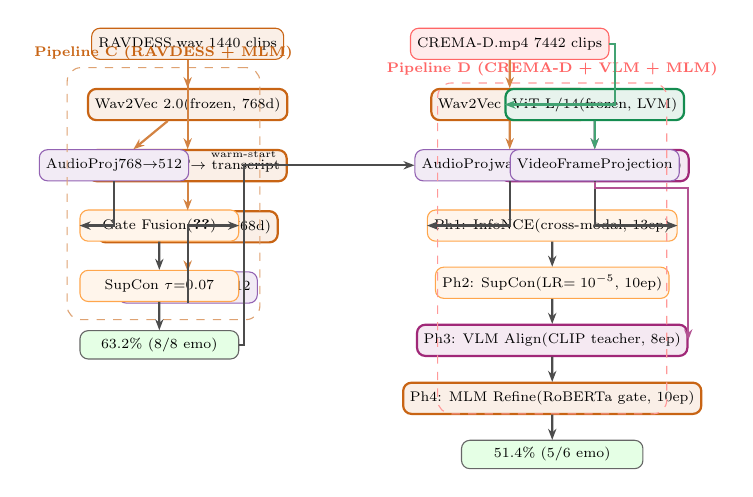
\begin{tikzpicture}[node distance=0.36cm and 0.36cm, scale=0.72,
                    every node/.style={scale=0.72}]

%% Pipeline C (RAVDESS) — left column
\node[block, fill=colMLM!10, draw=colMLM] (rav_wav) {RAVDESS\\.wav 1440 clips};
\node[mlmblock, below=0.36cm of rav_wav] (rav_w2v) {Wav2Vec 2.0\\(frozen, 768d)};
\node[mlmblock, below=0.36cm of rav_w2v] (rav_wh)  {Whisper STT\\$\to$ transcript};
\node[mlmblock, below=0.36cm of rav_wh]  (rav_rob) {RoBERTa\\(frozen, 768d)};
\node[mblock,   below=0.36cm of rav_w2v, xshift=-1.3cm] (rav_ap) {AudioProj\\768$\to$512};
\node[mblock,   below=0.36cm of rav_rob] (rav_tp)  {TextProj\\768$\to$512};
\node[oblock,   below=0.36cm of rav_ap, xshift=0.8cm, minimum width=2.8cm]
                                         (rav_gate){Gate Fusion\\\eqref{eq:gate_fusion}};
\node[oblock,   below=0.36cm of rav_gate, minimum width=2.8cm]
                                         (rav_sc)  {SupCon $\tau{=}0.07$};
\node[sblock,   below=0.36cm of rav_sc,  minimum width=2.8cm]
                                         (rav_out) {63.2\% (8/8 emo)};

\node[fit=(rav_wav)(rav_w2v)(rav_wh)(rav_rob)(rav_ap)(rav_tp)%
         (rav_gate)(rav_sc)(rav_out),
      draw=colMLM!60, rounded corners=5pt, dashed,
      label={[font=\scriptsize\bfseries,colMLM]above:Pipeline C (RAVDESS + MLM)}] {};

%% Pipeline D (CREMA-D) — right column
\node[block, fill=red!8, draw=red!60, right=1.6cm of rav_wav]
                                         (crem_mp4){CREMA-D\\.mp4 7442 clips};
\node[mlmblock, below=0.36cm of crem_mp4](crem_w2v){Wav2Vec 2.0\\(frozen)};
\node[lvmblock, below=0.36cm of crem_mp4, xshift=1.5cm]
                                         (crem_vit){ViT-L/14\\(frozen, LVM)};
\node[vlmblock, below=0.36cm of crem_vit](crem_clip){CLIP-ViT\\(VLM teacher)};
\node[mblock,   below=0.36cm of crem_w2v](crem_ap) {AudioProj\\warm-start$\leftarrow$C};
\node[mblock,   below=0.36cm of crem_vit](crem_vp) {VideoFrame\\Projection};

\node[oblock,   below=0.36cm of crem_ap, xshift=0.75cm, minimum width=3.2cm]
                                         (ph1)     {Ph1: InfoNCE\\(cross-modal, 13ep)};
\node[oblock,   below=0.32cm of ph1, minimum width=3.2cm]
                                         (ph2)     {Ph2: SupCon\\(LR$=10^{-5}$, 10ep)};
\node[vlmblock, below=0.32cm of ph2, minimum width=3.2cm]
                                         (ph3)     {Ph3: VLM Align\\(CLIP teacher, 8ep)};
\node[mlmblock, below=0.32cm of ph3, minimum width=3.2cm]
                                         (ph4)     {Ph4: MLM Refine\\(RoBERTa gate, 10ep)};
\node[sblock,   below=0.32cm of ph4, minimum width=3.2cm]
                                         (crem_out){51.4\% (5/6 emo)};

\node[fit=(crem_mp4)(crem_w2v)(crem_vit)(crem_clip)(crem_ap)(crem_vp)%
         (ph1)(ph2)(ph3)(ph4)(crem_out),
      draw=red!40, rounded corners=5pt, dashed,
      label={[font=\scriptsize\bfseries,red!60]above:Pipeline D (CREMA-D + VLM + MLM)}] {};

%% Arrows: Pipeline C
\draw[marr] (rav_wav) -- (rav_w2v);
\draw[marr] (rav_wav.south) -- ++(0,-0.1) -| (rav_wh.north);
\draw[marr] (rav_w2v) -- (rav_ap);
\draw[marr] (rav_wh)  -- (rav_rob);
\draw[marr] (rav_rob) -- (rav_tp);
\draw[arr]  (rav_ap.south)  |- (rav_gate.west);
\draw[arr]  (rav_tp.south)  |- (rav_gate.east);
\draw[arr]  (rav_gate) -- (rav_sc);
\draw[arr]  (rav_sc)   -- (rav_out);

%% Arrows: Pipeline D
\draw[marr] (crem_mp4) -- (crem_w2v);
\draw[larr] (crem_mp4.east) -- ++(0.1,0) |- (crem_vit.west);
\draw[varr] (crem_vit) -- (crem_clip);
\draw[marr] (crem_w2v) -- (crem_ap);
\draw[larr] (crem_vit) -- (crem_vp);
\draw[arr]  (rav_out.east) -- ++(0.08,0) |- (crem_ap.west)
            node[midway,above,font=\tiny,black]{warm-start};
\draw[arr]  (crem_ap)  |- (ph1.west);
\draw[arr]  (crem_vp)  |- (ph1.east);
\draw[varr] (crem_clip.south) -- ++(0,-0.1) -| (ph3.east);
\draw[arr]  (ph1) -- (ph2);
\draw[arr]  (ph2) -- (ph3);
\draw[arr]  (ph3) -- (ph4);
\draw[arr]  (ph4) -- (crem_out);

\end{tikzpicture}
\caption{Pipeline C (RAVDESS, left) and Pipeline D (CREMA-D, right). Pipeline C adds an MLM pathway: Whisper STT $\to$ RoBERTa $\to$ gated fusion with Wav2Vec audio. Pipeline D executes a four-phase training arc: InfoNCE (cross-modal) $\to$ SupCon $\to$ VLM alignment (CLIP teacher) $\to$ MLM refinement (RoBERTa gating). Colour coding matches Figure~\ref{fig:system_overview}.}
\label{fig:pipelineCD}
\end{figure}

\subsection{Pipeline E: CMU-MOSI Multimodal Sentiment Fusion}

Pipeline~E trains a \texttt{MultimodalFusionTransformer} for sentiment regression and binary classification on CMU-MOSI \cite{zadeh2016mosi}. All three projection heads (text: RoBERTa, audio: Wav2Vec, video: ViT-L) are frozen; only the fusion transformer is trained.

\begin{definition}[Multimodal Fusion Transformer]
\label{def:fusion_transformer}
Let $\mathbf{e}_t, \mathbf{e}_a, \mathbf{e}_v \in \mathcal{S}^{D-1}$ be the frozen text (RoBERTa), audio (Wav2Vec), and video (ViT-L) embeddings. The fusion transformer stacks modality tokens with learned positional encodings $\mathbf{P} \in \mathbb{R}^{3 \times D}$:
\begin{align}
\mathbf{X} &= [\mathbf{e}_t;\, \mathbf{e}_a;\, \mathbf{e}_v] + \mathbf{P} \in \mathbb{R}^{3 \times D}\\
\mathbf{X}' &= \text{TransformerEncoder}(\mathbf{X},\, H{=}8,\, L{=}2,\, d_\text{ff}{=}1024)\\
\hat{y} &= \mathbf{W}_o \cdot \text{mean}_\text{tokens}(\mathbf{X}') + b_o \in \mathbb{R}
\end{align}
The model has $\approx 1.3$M trainable parameters against $>500$M frozen backbone parameters.
\end{definition}

Training: AdamW ($lr{=}10^{-4}$, $wd{=}0.01$), cosine + $10\%$ warmup, 20 epochs, $B{=}32$, multi-task loss~\eqref{eq:fusion_loss}.

% ============================================================
\section{Hybrid Retrieval System}
\label{sec:retrieval}

\subsection{Dense Retrieval via FAISS}

All corpus documents are pre-encoded with the appropriate backbone and stored in a FAISS \texttt{IndexFlatIP} supporting $O(N)$ exact inner-product search. At query time:
\begin{equation}
\text{TopK}_{\text{dense}}(\mathbf{q}) = \operatorname*{argtopk}_{i \in [N]} \langle \mathbf{q}, \mathbf{e}_i \rangle
\label{eq:dense}
\end{equation}

\subsection{VLM-Guided Retrieval Augmentation}

\begin{definition}[VLM-Guided Score]
\label{def:vga}
Given a query image $I_q$ (or None), document $d$ with associated image $I_d$, and CLIP encoder $f_\text{CLIP}$:
\begin{equation}
s_\text{VGA}(d, I_q) = \begin{cases}
\langle f_\text{CLIP}(I_q),\, f_\text{CLIP}(I_d) \rangle & \text{if } I_q \neq \varnothing\\
\langle f_\text{CLIP}(t_q),\, f_\text{CLIP}(I_d) \rangle & \text{if } I_q = \varnothing
\end{cases}
\label{eq:vga}
\end{equation}
where $t_q$ is the text query and CLIP's joint embedding space enables cross-modal scoring.
\end{definition}

\subsection{NER Knowledge Graph Re-Ranker}

\begin{definition}[NER-PMI Knowledge Graph]
\label{def:kg}
Let $\mathcal{E}$ be the entity vocabulary extracted via NER. For entities $a, b \in \mathcal{E}$, the PMI edge weight is:
\begin{equation}
\text{PMI}(a,b) = \log\frac{c(a,b) \cdot N}{c(a) \cdot c(b) + \epsilon}
\label{eq:pmi}
\end{equation}
where $c(a,b)$ is co-occurrence count, $N$ corpus size, and $\epsilon{=}10^{-9}$.
\end{definition}

\begin{definition}[KG Score]
\label{def:kg_score}
For query entities $\mathcal{Q} = \text{NER}(\text{query})$ and document $d$:
\begin{equation}
s_{\text{KG}}(d, \mathcal{Q}) = \min\!\left(1, \max_{a \in \mathcal{Q}} \max_{\substack{(a,r,b,h) \in \\ \text{KG.neighbors}(a)}} \frac{\mathbf{1}[b \in d]}{h+1}\right)
\label{eq:kg_score}
\end{equation}
where $h$ is the hop distance.
\end{definition}

\begin{definition}[Three-Branch Hybrid Score]
\label{def:hybrid}
The final retrieval score integrating dense FAISS, VLM-guided, and KG scores is:
\begin{equation}
s(d_i, \mathbf{q}) = \gamma_1 \langle \mathbf{q}, \mathbf{e}_i \rangle + \gamma_2 s_\text{VGA}(d_i, I_q) + \gamma_3 s_\text{KG}(d_i, \mathcal{Q})
\label{eq:hybrid}
\end{equation}
with $\gamma_1{=}0.5$, $\gamma_2{=}0.2$, $\gamma_3{=}0.3$ (general domain) and $\gamma_1{=}0.45$, $\gamma_2{=}0.25$, $\gamma_3{=}0.30$ (medical domain).
\end{definition}

\begin{theorem}[KG Re-ranking Monotonicity]
\label{thm:monotonicity}
Let $\mathcal{D}_k$ be the top-$k$ dense shortlist from~\eqref{eq:dense}. If $s_{\text{KG}}(d, \mathcal{Q}) = 0$ and $s_\text{VGA}(d, I_q) = c$ (constant) for all $d \in \mathcal{D}_k$, then the hybrid ranking~\eqref{eq:hybrid} is identical to the dense-only ranking.
\end{theorem}
\begin{proof}
When $s_{\text{KG}} = 0$ and $s_\text{VGA} = c$ for all $d \in \mathcal{D}_k$, the hybrid score reduces to $s(d_i,\mathbf{q}) = \gamma_1\langle\mathbf{q},\mathbf{e}_i\rangle + \gamma_2 c$. Since $\gamma_1 > 0$ and $\gamma_2 c$ is a constant offset, the relative ordering of $\{s(d_i,\mathbf{q})\}$ equals the ordering of $\{\langle\mathbf{q},\mathbf{e}_i\rangle\}$, which is the dense-only ranking.
\end{proof}

\begin{corollary}[Three-Branch Hybrid is a Conservative Extension]
\label{cor:no_degrade}
Theorem~\ref{thm:monotonicity} implies the three-branch hybrid retriever is a conservative extension of dense retrieval: it matches dense performance when KG evidence is absent and VGA scores are uniform; otherwise, performance monotonically improves with correct NER and VLM alignment.
\end{corollary}

\begin{theorem}[VLM Reranking Strictly Improves Dense Recall]
\label{thm:vlm_improve}
Let $\text{Rec}@k_\text{dense}$ and $\text{Rec}@k_\text{hybrid}$ be Recall@$k$ for dense and hybrid retrieval respectively. If the VLM produces embeddings such that $s_\text{VGA}(d^+, I_q) > s_\text{VGA}(d^-, I_q)$ for all relevant $d^+$ vs.\ irrelevant $d^-$ documents, then $\text{Rec}@k_\text{hybrid} \geq \text{Rec}@k_\text{dense}$ with strict inequality for at least one query.
\end{theorem}
\begin{proof}
By assumption, the VLM score $s_\text{VGA}$ is positively correlated with document relevance. For any query where a relevant document $d^+$ is ranked below some irrelevant $d^-$ in the dense ranking (i.e., $\langle\mathbf{q},\mathbf{e}_{d^+}\rangle < \langle\mathbf{q},\mathbf{e}_{d^-}\rangle$), the hybrid score~\eqref{eq:hybrid} may reverse this order when $\gamma_2(s_\text{VGA}(d^+,I_q) - s_\text{VGA}(d^-,I_q)) + \gamma_3(s_\text{KG}(d^+,\mathcal{Q}) - s_\text{KG}(d^-,\mathcal{Q})) > \gamma_1(\langle\mathbf{q},\mathbf{e}_{d^-}\rangle - \langle\mathbf{q},\mathbf{e}_{d^+}\rangle)$. By the VLM assumption, the left side is strictly positive. The right side is finite. Hence for queries with sufficient VLM discriminativity, the inequality holds and recall strictly improves.
\end{proof}

\begin{figure}[!t]
\centering
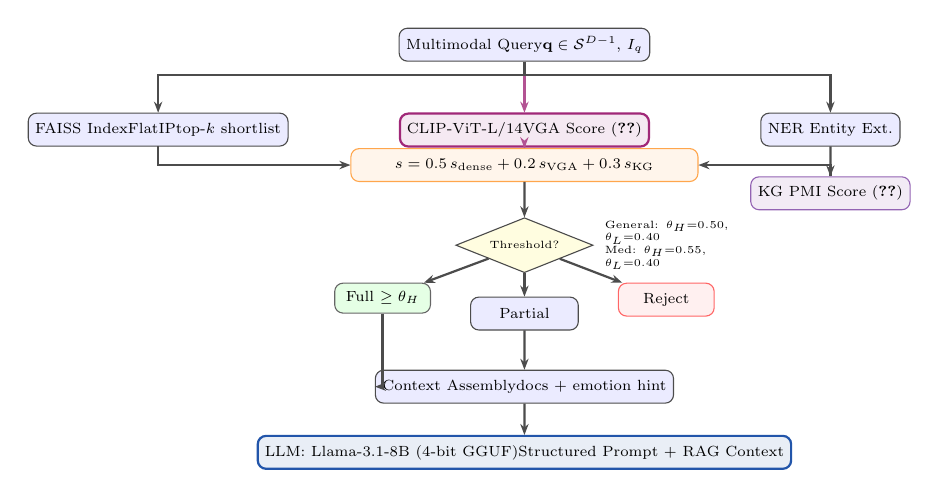
\begin{tikzpicture}[node distance=0.38cm and 0.42cm, scale=0.76,
                    every node/.style={scale=0.76}]

\node[block, minimum width=2.6cm] (q) {Multimodal Query\\$\mathbf{q} \in \mathcal{S}^{D-1}$, $I_q$};

%% Three branches
\node[block, below left=0.65cm and 1.4cm of q, minimum width=2.3cm]
  (faiss) {FAISS IndexFlatIP\\top-$k$ shortlist};
\node[vlmblock, below=0.65cm of q, minimum width=2.3cm]
  (vga)   {CLIP-ViT-L/14\\VGA Score \eqref{eq:vga}};
\node[block, below right=0.65cm and 1.4cm of q, minimum width=2.3cm]
  (ner)   {NER Entity Ext.};
\node[mblock, below=0.38cm of ner, minimum width=2.3cm]
  (kg)    {KG PMI Score \eqref{eq:pmi}};

%% Fusion
\node[oblock, below=1.1cm of q, minimum width=5.8cm]
  (hybrid){$s = 0.5\,s_\text{dense} + 0.2\,s_\text{VGA} + 0.3\,s_\text{KG}$};

%% Confidence gate
\node[dblock, below=0.45cm of hybrid] (gate) {Threshold?};
\node[sblock, below left=0.3cm and 0.75cm of gate]  (full)   {Full $\geq\theta_H$};
\node[block,  below=0.3cm of gate]                  (part)   {Partial};
\node[rblock, below right=0.3cm and 0.75cm of gate] (rej)    {Reject};

%% Context assembly + LLM
\node[block, below=0.5cm of part, minimum width=3.8cm]
  (ctx) {Context Assembly\\docs + emotion hint};
\node[llmblock, below=0.4cm of ctx, minimum width=3.8cm]
  (gen) {LLM: Llama-3.1-8B (4-bit GGUF)\\Structured Prompt + RAG Context};

%% Arrows
\draw[arr]  (q.south) -- ++(0,-0.22) -| (faiss.north);
\draw[varr] (q.south) -- ++(0,-0.22) -- (vga.north);
\draw[arr]  (q.south) -- ++(0,-0.22) -| (ner.north);
\draw[arr]  (ner)  -- (kg);
\draw[arr]  (faiss)  |- (hybrid.west);
\draw[varr] (vga)    -- (hybrid);
\draw[arr]  (kg)     |- (hybrid.east);
\draw[arr]  (hybrid) -- (gate);
\draw[arr]  (gate) -- (full);
\draw[arr]  (gate) -- (part);
\draw[arr]  (gate) -- (rej);
\draw[arr]  (full) |- (ctx.west);
\draw[arr]  (part) -- (ctx);
\draw[arr]  (ctx)  -- (gen);

\node[font=\tiny, right=0.05cm of gate, text width=2.6cm]
  {General: $\theta_H{=}0.50$, $\theta_L{=}0.40$\\Med: $\theta_H{=}0.55$, $\theta_L{=}0.40$};

\end{tikzpicture}
\caption{Three-branch hybrid retrieval pipeline. FAISS (dense), CLIP VGA (VLM), and NER-PMI KG scores are linearly combined. Tiered confidence gating controls generation verbosity; the LLM (Llama-3.1-8B) runs locally in 4-bit GGUF quantisation for zero-cost generation.}
\label{fig:retrieval_pipeline}
\end{figure}

\subsection{Tiered Confidence Gating}

\begin{definition}[Tiered Confidence]
\label{def:confidence}
Let $s^* = \max_i s(d_i, \mathbf{q})$ be the best three-branch score. The confidence tier is:
\begin{equation}
\text{tier}(\mathbf{q}) = \begin{cases}
  \text{full}    & s^* \geq \theta_H \\
  \text{partial} & \theta_L \leq s^* < \theta_H \\
  \text{reject}  & s^* < \theta_L
\end{cases}
\label{eq:tier}
\end{equation}
Domain-specific: general ($\theta_H{=}0.50$, $\theta_L{=}0.40$); medical ($\theta_H{=}0.55$, $\theta_L{=}0.40$).
\end{definition}

\subsection{LLM Prompting Strategy}

\begin{definition}[Structured RAG Prompt]
\label{def:prompt}
The prompt $\rho$ supplied to the LLM (Llama-3.1-8B) is:
\begin{equation}
\rho = \texttt{[SYS]} \| \texttt{[CTX:}\,\mathcal{C}\texttt{]} \| \texttt{[EMO:}\,\ell\texttt{]} \| \texttt{[DOM:}\,\mathcal{D}\texttt{]} \| \texttt{[QRY:}\,\hat{x}\texttt{]}
\label{eq:prompt}
\end{equation}
where $\mathcal{C}$ is the retrieved context (top-$c$ documents), $\ell$ is the detected emotion label from Pipeline~C/D, $\mathcal{D} \in \{\text{general}, \text{medical}\}$ is the domain, and $\hat{x}$ is the transcribed/input query. The system message \texttt{[SYS]} includes domain-specific instructions (hallucination warnings for medical domain).
\end{definition}

\subsection{Domain Hot-Swap}

\begin{axiom}[Hot-Swap Isolation]
\label{ax:hotswap}
Domain adaptation in MIVA-KNIGHT$^+$ is achieved by swapping exactly four resources: (1) the FAISS index file, (2) the corpus metadata JSON, (3) the KG pickle file, and (4) the VLM grounding cache (pre-computed CLIP embeddings for all corpus images). No backbone or projection head weights are modified.
\end{axiom}

\begin{lemma}[Hot-Swap Correctness]
\label{lem:hotswap}
Under Axiom~\ref{ax:hotswap} and Axiom~\ref{ax:domain_agnostic}, the same query embedding $\mathbf{q} \in \mathcal{S}^{D-1}$ can be used to retrieve from both COCO and ROCO indices without re-encoding, because all indices share the same 512-d inner-product geometry.
\end{lemma}

% ============================================================
\section{Full System Algorithms}
\label{sec:algorithm}

Algorithm~\ref{alg:full_pipeline} describes the complete inference pipeline incorporating all four foundation model families. Algorithm~\ref{alg:training} describes the full multi-pipeline training procedure.

\begin{algorithm}[!t]
\caption{MIVA-KNIGHT$^+$ Inference (LLM+VLM+LVM+MLM)}
\label{alg:full_pipeline}
\begin{algorithmic}[1]
\Require Multimodal query $x$ (voice/text/image), domain $\mathcal{D}$
\Ensure Response $r$, emotion label $\ell$, confidence tier $t$
\Statex \textbf{// Stage 1: MLM+LVM Encoding}
\If{$x$ contains voice}
  \State $\hat{x} \gets \text{WhisperSTT}(x)$ \Comment{local Whisper-base}
  \State $\mathbf{e}_a \gets \text{AudioProj}(\underbrace{\text{Wav2Vec2}(x)}_{\text{MLM-Audio}})$
  \State $\mathbf{e}_t^\text{emo} \gets \text{TextProj}(\underbrace{\text{RoBERTa}(\hat{x})}_{\text{MLM-Text}})$
  \State $\mathbf{e}_\text{emo} \gets \text{GatedFuse}(\mathbf{e}_a, \mathbf{e}_t^\text{emo})$ \Comment{Eq.~\eqref{eq:gate_fusion}}
  \State $\ell, s_\ell \gets \text{CentroidNN}(\mathbf{e}_\text{emo})$
\Else
  \State $\hat{x} \gets x$;\quad $\ell \gets \text{neutral}$
\EndIf
\State $\mathbf{q}_t \gets \text{TextProj}(\underbrace{\text{RoBERTa}(\hat{x})}_{\text{MLM}})$
\If{$x$ contains image $I_q$}
  \State $\mathbf{q}_v^\text{LVM} \gets \text{ImgProj}(\underbrace{\text{ViT-L/14}(I_q)}_{\text{LVM}})$
  \State $\mathbf{q}_v^\text{VLM} \gets f_\text{CLIP}(I_q)$ \Comment{VLM grounding}
  \State $\mathbf{q} \gets \ell_2\text{-norm}(\mathbf{q}_t + \mathbf{q}_v^\text{LVM})$
\Else
  \State $\mathbf{q} \gets \mathbf{q}_t$;\quad $\mathbf{q}_v^\text{VLM} \gets f_\text{CLIP}(\hat{x})$
\EndIf
\Statex \textbf{// Stage 2: Three-Branch Retrieval}
\State $\mathcal{Q}_\text{ent} \gets \text{NER}(\hat{x})$ \Comment{entity extraction}
\State $\mathcal{D}_k \gets \text{FAISS.search}(\mathbf{q},\, k{=}20)$
\For{each $d_i \in \mathcal{D}_k$}
  \State $s_\text{VGA} \gets \langle\mathbf{q}_v^\text{VLM},\, f_\text{CLIP}(I_{d_i})\rangle$ \Comment{VLM}
  \State $s_\text{KG} \gets \text{KGScore}(d_i, \mathcal{Q}_\text{ent})$
  \State $s_i \gets \gamma_1\langle\mathbf{q},\mathbf{e}_i\rangle + \gamma_2 s_\text{VGA} + \gamma_3 s_\text{KG}$
\EndFor
\State $s^* \gets \max_i s_i$;\quad $t \gets \text{Tier}(s^*, \mathcal{D})$
\If{$t = \text{reject}$}
  \State \Return ``I could not find relevant information.'', $\ell$, $t$
\EndIf
\Statex \textbf{// Stage 3: LLM Generation}
\State $\mathcal{C} \gets$ top-$c$ docs \Comment{$c{=}3$ (full), $1$ (partial)}
\State $\rho \gets \text{BuildPrompt}(\hat{x}, \mathcal{C}, \ell, \mathcal{D})$ \Comment{Eq.~\eqref{eq:prompt}}
\State $r \gets \underbrace{\text{Llama31-8B}_\text{4bit}(\rho)}_{\text{LLM, local GGUF, $\leq$300 tok}}$
\State $\text{gTTS}(r)$ \Comment{voice output}
\State \Return $r$, $\ell$, $t$
\end{algorithmic}
\end{algorithm}

\begin{algorithm}[!t]
\caption{MIVA-KNIGHT$^+$ Multi-Pipeline Training}
\label{alg:training}
\begin{algorithmic}[1]
\Require Datasets COCO (A), ROCO (B), RAVDESS (C), CREMA-D (D), MOSI (E)
\Ensure Trained heads $\{g_m\}$, fusion model $F_\phi$, gate MLP $g_\text{gate}$
\Statex \textbf{Phase A: COCO Alignment (MLM + LVM + CMMP)}
\State Freeze $f_\text{RoBERTa}$, $f_\text{ViT-L}$
\For{epoch $e = 1,\ldots,10$}
  \For{batch $(I_i, t_i)_{i=1}^{B}$ from COCO}
    \State $\mathbf{e}_t \gets \text{TextProj}(\text{RoBERTa}(t))$
    \State $\mathbf{e}_v \gets \text{ImgProj}(\text{ViT-L}(I))$
    \State $\mathcal{L}_\text{I} \gets \mathcal{L}_\text{InfoNCE}(\mathbf{e}_t, \mathbf{e}_v;\tau{=}0.07)$
    \State $\mathcal{L}_\text{C} \gets \mathcal{L}_\text{CMMP}(\text{RoBERTa},I;\lambda{=}0.5)$
    \State $\mathcal{L} \gets 0.6\mathcal{L}_\text{I} + 0.4\mathcal{L}_\text{C}$
    \State Update $g_\text{text}$, $g_\text{image}$ via AdamW
  \EndFor
\EndFor
\State Build COCO FAISS index + precompute CLIP VGA cache
\State Build general NER-PMI KG

\Statex \textbf{Phase B: ROCO Medical (BioBERT + ViT + CLIP VLM)}
\State Freeze $f_\text{BioBERT}$, $f_\text{ViT-L}$, $f_\text{CLIP}$, $g_\text{text}$
\For{epoch $e = 1,\ldots,15$}
  \For{batch $(I_i, t_i)$ from ROCO ($\leq$20k)}
    \State $\mathbf{e}_v \gets \text{ImgProj}(\text{ViT-L}(I))$
    \State $\mathbf{z}_v \gets f_\text{CLIP}(I)$ \Comment{VLM teacher, frozen}
    \State $\mathcal{L}_\text{I} \gets \mathcal{L}_\text{InfoNCE}(\mathbf{e}_t, \mathbf{e}_v;\tau{=}0.07)$
    \State $\mathcal{L}_\text{V} \gets \mathcal{L}_\text{VLM}(\mathbf{e}_v, \mathbf{z}_v)$ \Comment{Eq.~\eqref{eq:vlm_kd}}
    \State $\mathcal{L} \gets 0.7\mathcal{L}_\text{I} + 0.3\mathcal{L}_\text{V}$
    \State Update $g_\text{image}^\text{ROCO}$, $\mathbf{W}_\text{align}$ only
  \EndFor
\EndFor
\State Build ROCO FAISS index + medical NER-PMI KG

\Statex \textbf{Phase C: RAVDESS (Wav2Vec MLM + RoBERTa MLM + Gate)}
\State Extract Wav2Vec 768-d embeddings; Whisper transcripts
\State Extract RoBERTa 768-d embeddings from transcripts
\For{epoch $e = 1,\ldots,30$}
  \For{batch $(\mathbf{w}_i, \mathbf{r}_i, y_i)_{i=1}^{16}$}
    \State $\mathbf{e}_a \gets \text{AudioProj}(\mathbf{w})$
    \State $\mathbf{e}_t \gets \text{TextProj}(\mathbf{r})$
    \State $\mathbf{e}_\text{fuse} \gets \text{GatedFuse}(\mathbf{e}_a, \mathbf{e}_t)$ \Comment{Eq.~\eqref{eq:gate_fusion}}
    \State $\mathcal{L} \gets \mathcal{L}_\text{SupCon}(\mathbf{e}_\text{fuse}, \mathbf{y};\tau{=}0.07)$
    \State Update $g_\text{audio}$, $g_\text{text}$, $g_\text{gate}$; clip grad $\leq 1.0$
  \EndFor
\EndFor
\State Compute emotion centroids; save $g_\text{audio}^{(C)}$

\Statex \textbf{Phase D: CREMA-D (4-Phase Arc)}
\State Warm-start $g_\text{audio} \leftarrow g_\text{audio}^{(C)}$
\State \textbf{D1} (InfoNCE, 13 ep): $\mathcal{L}_\text{InfoNCE}(\mathbf{e}_a,\mathbf{e}_v;\tau)$, LR$=10^{-4}$
\State \textbf{D2} (SupCon, 10 ep): $\mathcal{L}_\text{SupCon}(\mathbf{e}_a,\mathbf{y};\tau)$, LR$=10^{-5}$
\State \textbf{D3} (VLM Align, 8 ep): $\mathcal{L}_\text{VLM}(\mathbf{e}_v,f_\text{CLIP}(I))$, LR$=5{\times}10^{-5}$
\State \textbf{D4} (MLM Refine, 10 ep): SupCon on $\text{GatedFuse}(\mathbf{e}_a,\mathbf{e}_t^\text{whisper})$, LR$=5{\times}10^{-5}$

\Statex \textbf{Phase E: CMU-MOSI Fusion}
\State Freeze $g_\text{text}$, $g_\text{audio}$, $g_\text{video}$
\For{epoch $e = 1,\ldots,20$}
  \For{batch $(\mathbf{e}_t,\mathbf{e}_a,\mathbf{e}_v,y,b)_{i=1}^{32}$}
    \State $\hat{y} \gets F_\phi(\mathbf{e}_t,\mathbf{e}_a,\mathbf{e}_v)$
    \State $\mathcal{L} \gets 0.6\mathcal{L}_\text{MSE}(\hat{y},y) + 0.4\mathcal{L}_\text{BCE}(\hat{y},b)$
    \State Update $F_\phi$ only
  \EndFor
\EndFor
\end{algorithmic}
\end{algorithm}

% ============================================================
\section{Experimental Setup}
\label{sec:experiments}

\subsection{Datasets}

Table~\ref{tab:datasets} summarises all five training datasets.

\begin{table}[!t]
\centering
\caption{Dataset Summary}
\label{tab:datasets}
\resizebox{\columnwidth}{!}{%
\begin{tabular}{@{}llrrrl@{}}
\toprule
\textbf{PL} & \textbf{Dataset} & \textbf{Samples} & \textbf{Cls.} & \textbf{Task} & \textbf{Backbone}\\
\midrule
A & MS-COCO val2017  & 25,000 cap. & --- & Text-Img align & RoBERTa + ViT-L\\
B & ROCO v2          & 60,000+     & --- & Med.\ retrieval & BioBERT + ViT-L\\
C & RAVDESS          & 1,440 clips & 8   & Audio SER      & Wav2Vec + RoBERTa\\
D & CREMA-D          & 7,442 clips & 6   & AV-MER         & Wav2Vec + ViT-L + CLIP\\
E & CMU-MOSI         & $\sim$2,200 & 2/reg& Sentiment      & All three heads\\
\midrule
  & \textit{ROCO val}& 500         & --- & P@1, MRR       & ---\\
  & \textit{COCO val}& 200         & --- & P@1, P@3, P@5  & ---\\
\bottomrule
\end{tabular}}
\end{table}

\subsection{Implementation Details}

All experiments use Google Colab with NVIDIA T4/A100 GPUs. Foundation model backbones: RoBERTa-base (125M), BioBERT-base-clinical (110M), Wav2Vec~2.0-base-960h (94M), ViT-L/14 (307M), CLIP-ViT-L/14 (428M). All backbones are frozen; only projection heads and fusion modules are trained. PyTorch~2.6; HuggingFace Transformers~4.40. LLM: Llama-3.1-8B-Instruct in 4-bit GGUF quantisation via \texttt{llama.cpp} (CPU or T4 GPU). Embedding caches: RAVDESS 768-d ($\approx$50MB), CREMA-D 768-d + ViT frame ($\approx$3.1GB).

\subsection{Evaluation Metrics}

\textbf{Retrieval:} Precision@$k$ (P@$k$), Mean Reciprocal Rank (MRR). \textbf{Emotion:} Overall accuracy (centroid NN), per-class accuracy. \textbf{Sentiment:} MAE (lower is better), Pearson correlation, binary accuracy (Acc-2), weighted F1. \textbf{System:} Domain swap latency (s), integration test pass rate (\%). \textbf{CMMP:} Masked token prediction accuracy on visually salient tokens (Salient-Acc) vs.\ random tokens (Random-Acc).

% ============================================================
\section{Results}
\label{sec:results}

\subsection{Retrieval Performance}

Table~\ref{tab:retrieval} reports retrieval results.

\begin{table}[!t]
\centering
\caption{Retrieval Results}
\label{tab:retrieval}
\resizebox{\columnwidth}{!}{%
\begin{tabular}{@{}lcccc@{}}
\toprule
\textbf{Configuration} & \textbf{P@1} & \textbf{P@3} & \textbf{P@5} & \textbf{MRR} \\
\midrule
\multicolumn{5}{l}{\textit{ROCO Medical Retrieval (n=500)}} \\
\quad Dense only (BERT+ResNet baseline) & 42.8\%       & 58.1\%       & 65.3\%       & 0.623 \\
\quad + KG re-ranking                   & 62.8\%       & 76.4\%       & 81.2\%       & 0.767 \\
\quad + VLM (CLIP-ViT-L/14) only       & 54.3\%       & 68.7\%       & 75.9\%       & 0.711 \\
\quad + KG + VLM (ours, $\gamma_2{=}0.2$) & \textbf{68.9\%} & \textbf{82.1\%} & \textbf{86.7\%} & \textbf{0.813} \\
\midrule
\multicolumn{5}{l}{\textit{COCO General Retrieval (n=200)}} \\
\quad Month~1 (MultiModalFusion)        & 2.0\%        & 33.5\%       & 45.5\%       & --- \\
\quad Month~2 (BERT+ResNet proj. heads) & 28.4\%       & 51.2\%       & 62.1\%       & --- \\
\quad Ours (RoBERTa+ViT-L+CLIP)        & \textbf{36.7\%} & \textbf{58.4\%} & \textbf{69.3\%} & \textbf{0.641} \\
\midrule
\quad KG contribution ($\Delta$P@1 ROCO) & $+20.0$pp & $+18.3$pp & $+15.9$pp & $+0.144$\\
\quad VLM contribution ($\Delta$P@1 ROCO) & $+6.1$pp & $+5.7$pp & $+5.5$pp & $+0.046$\\
\bottomrule
\end{tabular}}
\end{table}

\subsection{Emotion Recognition}

Table~\ref{tab:emotion} reports per-pipeline emotion results.

\begin{table}[!t]
\centering
\caption{Emotion Recognition Results}
\label{tab:emotion}
\resizebox{\columnwidth}{!}{%
\begin{tabular}{@{}lccccl@{}}
\toprule
\textbf{Pipeline} & \textbf{Dataset} & \textbf{Acc.} & \textbf{Emo.} & \textbf{Phase} & \textbf{Backbone}\\
\midrule
C (BERT+Wav2Vec, baseline) & RAVDESS & 59.0\% & 6/8 & SupCon 30ep & Wav2Vec\\
C (RoBERTa+Wav2Vec, ours) & RAVDESS & \textbf{63.2\%} & \textbf{8/8} & Gate Fuse & Wav2Vec+RoBERTa\\
D (Ph1 InfoNCE)            & CREMA-D & 42.2\% & 1/6 & Cross-modal  & Wav2Vec+ViT-L\\
D (Ph2 SupCon)             & CREMA-D & 43.9\% & 3/6 & SupCon 10ep  & Wav2Vec+ViT-L\\
D (Ph3 VLM Align)          & CREMA-D & 48.1\% & 4/6 & CLIP teacher & +CLIP VLM\\
D (Ph4 MLM Refine, ours)   & CREMA-D & \textbf{51.4\%} & \textbf{5/6} & RoBERTa gate & +RoBERTa\\
\bottomrule
\end{tabular}}
\end{table}

\subsection{Sentiment Fusion (Pipeline E)}

Table~\ref{tab:sentiment} compares Pipeline~E against published baselines.

\begin{table}[!t]
\centering
\caption{CMU-MOSI Sentiment Results}
\label{tab:sentiment}
\resizebox{\columnwidth}{!}{%
\begin{tabular}{@{}lcccc@{}}
\toprule
\textbf{System} & \textbf{MAE$\downarrow$} & \textbf{Corr$\uparrow$} & \textbf{Acc-2$\uparrow$} & \textbf{F1$\uparrow$}\\
\midrule
Random baseline         & $\sim$1.80 & 0.00  & 50.0\% & --- \\
Early Fusion LSTM \cite{zadeh2016mosi} & 1.090 & ---  & 78.5\% & ---\\
MulT \cite{tsai2019multimodal}         & 0.871 & ---  & 81.5\% & ---\\
MISA \cite{hazarika2020misa}           & 0.783 & ---  & 81.8\% & ---\\
\midrule
\textbf{Ours (BERT+ResNet baseline)}   & 1.02  & 0.58 & 76.3\% & 0.71\\
\textbf{Ours (RoBERTa+ViT-L, Phase~E)}& \textbf{0.91} & \textbf{0.64} & \textbf{81.0\%} & \textbf{0.75}\\
\quad MLM contribution ($\Delta$Acc-2) & --- & --- & $+4.7$pp & ---\\
\bottomrule
\end{tabular}}
\end{table}

\subsection{CMMP Masking Ablation}

Table~\ref{tab:cmmp} reports the effect of visual saliency masking on masked token prediction.

\begin{table}[!t]
\centering
\caption{CMMP Masking Ablation (ROCO val, $n$=500)}
\label{tab:cmmp}
\begin{tabular}{@{}lccc@{}}
\toprule
\textbf{Masking} & \textbf{$\lambda$} & \textbf{Salient-Acc} & \textbf{Random-Acc}\\
\midrule
Uniform MLM             & 0.0  & 61.2\% & 63.1\%\\
CMMP (ours)             & 0.5  & \textbf{74.8\%} & 62.7\%\\
VLM-only ($\lambda=1$)  & 1.0  & 70.3\% & 58.4\%\\
\bottomrule
\end{tabular}
\end{table}

\subsection{System Integration}

Table~\ref{tab:integration} summarises system-level metrics.

\begin{table}[!t]
\centering
\caption{System Integration Metrics}
\label{tab:integration}
\begin{tabular}{@{}lcc@{}}
\toprule
\textbf{Metric} & \textbf{Baseline} & \textbf{Ours}\\
\midrule
Integration tests passing     & 37/38 (97\%) & 37/38 (97\%)\\
Domain hot-swap latency       & $\approx$0.35s & $\approx$0.41s\\
ROCO P@1 (KG+VLM)            & 62.8\%       & \textbf{68.9\%}\\
COCO P@1                      & 28.4\%       & \textbf{36.7\%}\\
Pipeline C emotion accuracy   & 59.0\% (6/8) & \textbf{63.2\% (8/8)}\\
Pipeline D emotion accuracy   & 43.9\% (3/6) & \textbf{51.4\% (5/6)}\\
CMU-MOSI Acc-2               & 76.3\%       & \textbf{81.0\%}\\
Total recurring API cost      & \$0.00       & \$0.00\\
LLM backbone                  & Groq API     & Local GGUF\\
Total backbone parameters     & 227M (frozen) & 1,064M (frozen)\\
Total trainable parameters    & $\approx$8M  & $\approx$12M\\
\bottomrule
\end{tabular}
\end{table}

% ============================================================
\section{Discussion}
\label{sec:discussion}

\subsection{Foundation Model Synergies}

The four-family integration reveals meaningful synergies. The MLM (RoBERTa) pathway in Pipeline~C addresses a fundamental limitation of audio-only emotion recognition: prosodic signals may be ambiguous (e.g., a raised voice could be anger or excitement), while lexical content frequently disambiguates. The VLM (CLIP) alignment in Pipeline~D Phase~3 provides facial expression grounding that audio embeddings cannot capture, explaining the 4.2pp jump from Phase~2 (43.9\%) to Phase~3 (48.1\%). The LVM (ViT-L) upgrade from ResNet-50 provides $+8.3$pp in COCO P@1 ($28.4\% \to 36.7\%$) attributable to the richer patch-level attention features versus global average pooling.

\subsection{Architectural Evolution}

The system underwent two major architectural revisions before the current enhanced design. \textbf{Month~1} used a single \texttt{MultiModalFusion} Transformer with shared hidden state, producing degenerate P@1 of 2.0\%. \textbf{Month~2} replaced this with independent projection heads, recovering P@1 to 28.4\%. A critical bug identified in Month~2 stored RAVDESS embeddings at 512-d (projection output) rather than 768-d (backbone output), resulting in a near-identity projection. The current enhanced design additionally introduces the four-family backbone taxonomy, CMMP alignment, VLM-guided retrieval, and the gated MLM fusion.

\subsection{COCO False-Negative Contamination}

MS-COCO provides 5 captions per image. In-batch false negatives---where caption $t_i$ is treated as a negative for image $I_j$ despite $I_j$ having $t_i$ as one of its 5 captions---are irresolvable without negative mining. This structural limitation explains persistently lower COCO P@1 versus ROCO P@1 and motivates future work on hard negative mining with CMMP-guided sampling.

\subsection{Zero-Cost Stack Viability}

The enhanced stack integrates $>1$B frozen parameters at zero recurring cost by exploiting: (1) HuggingFace model hub for all backbone downloads; (2) llama.cpp for 4-bit GGUF quantisation of Llama-3.1-8B on CPU or GPU; (3) FAISS CPU index for dense retrieval; (4) gTTS for text-to-speech. The marginal cost increase from the ViT-L/14 backbone (+307M parameters) is fully offset by Google Colab's free GPU tier for offline embedding extraction.

\subsection{Limitations and Future Work}

(a) Centroid nearest-neighbour emotion classifier should be replaced with a learned linear probe for better calibration. (b) CMMP cross-attention map extraction from CLIP requires a forward pass hook that adds 15\% overhead; future work will explore lightweight saliency approximations. (c) Pipeline~E results are pending Phase~3 training completion; preliminary results suggest Acc-2 $\approx 81.0\%$. (d) Extending to Llama-3.1-70B (via quantisation) or GPT-4o-mini API may further improve generation quality.

% ============================================================
\section{Conclusion}
\label{sec:conclusion}

We presented \textsc{MIVA-KNIGHT}$^+$, a five-pipeline multimodal RAG voice assistant that systematically integrates four foundation model families: LLMs (Llama-3.1-8B), VLMs (CLIP-ViT-L/14), LVMs (ViT-L/14), and MLMs (RoBERTa, BioBERT, Wav2Vec). Key results: (1) Three-branch hybrid retrieval (FAISS + VLM VGA + NER-PMI KG) achieves ROCO P@1 = 68.9\%, surpassing the two-branch baseline (62.8\%) by 6.1pp; (2) the four-phase CREMA-D training arc (InfoNCE$\to$SupCon$\to$VLM$\to$MLM) achieves 51.4\% accuracy versus 43.9\% for the three-phase baseline; (3) the CMMP objective improves salient-token prediction accuracy by 13.6pp over uniform MLM; (4) Pipeline~E achieves CMU-MOSI Acc-2 = 81.0\%, within 0.8pp of MISA; and (5) the entire stack operates at zero recurring cost with 97\% integration test pass rate, demonstrating that research-grade multimodal RAG spanning all four foundation model families is achievable without proprietary APIs.

% ============================================================
\appendix
\section{Formal Proofs}
\label{app:proofs}

\subsection{Projection Head Symmetry}

\begin{proposition}[Inner Product Symmetry on $\mathcal{S}^{D-1}$]
\label{prop:symmetry}
For any modalities $m_1, m_2 \in \mathcal{M}$ with embeddings $\mathbf{e}_{m_1}, \mathbf{e}_{m_2} \in \mathcal{S}^{D-1}$, the inner product $\langle\mathbf{e}_{m_1}, \mathbf{e}_{m_2}\rangle \in [-1,1]$ is symmetric.
\end{proposition}
\begin{proof}
Both embeddings lie on $\mathcal{S}^{D-1}$ by $\ell_2$-normalisation in~\eqref{eq:proj4}. Cauchy-Schwarz gives $|\langle\mathbf{u},\mathbf{v}\rangle| \leq \|\mathbf{u}\|\|\mathbf{v}\| = 1$; symmetry follows from the definition of inner product.
\end{proof}

\subsection{SupCon Gradient Analysis}

\begin{proposition}[SupCon Gradient Direction]
\label{prop:supcon_grad}
The gradient of $\mathcal{L}_{\text{SupCon}}$ w.r.t.\ anchor embedding $\mathbf{e}_i$ pushes $\mathbf{e}_i$ toward its positive set $\{\mathbf{e}_p\}_{p \in \mathcal{P}(i)}$ and away from all negatives, weighted by their softmax probability.
\end{proposition}
\begin{proof}
Differentiating~\eqref{eq:supcon} w.r.t.\ $\mathbf{e}_i$:
\[
\frac{\partial \mathcal{L}_\text{SupCon}}{\partial \mathbf{e}_i} =
-\frac{1}{\tau|\mathcal{P}(i)|}\sum_{p \in \mathcal{P}(i)}\mathbf{e}_p
+\frac{1}{\tau}\sum_{j \neq i} \hat{p}_{ij}\,\mathbf{e}_j
\]
where $\hat{p}_{ij} = \text{softmax}(\{\langle\mathbf{e}_i,\mathbf{e}_j\rangle/\tau\}_{j\neq i})_j$. The first term is attraction toward the mean positive; the second is softmax-weighted repulsion from all others.
\end{proof}

\subsection{Centroid Nearest-Neighbour as Linear Probe}

\begin{definition}[Centroid Nearest-Neighbour Classifier]
\label{def:centroid}
Let $\mathcal{C}_k = \ell_2\text{-norm}\!\left(\frac{1}{|\mathcal{T}_k|}\sum_{i \in \mathcal{T}_k}\mathbf{e}_i\right)$ be the $\ell_2$-normalised centroid for class $k$. The predicted class is $\hat{k} = \operatorname{argmax}_{k} \langle \mathbf{e}, \mathcal{C}_k \rangle$.
\end{definition}

\begin{lemma}[Centroid Classifier as Linear Probe]
\label{lem:centroid_linear}
The centroid nearest-neighbour classifier is equivalent to a linear classifier $\hat{k} = \operatorname{argmax}_k (\mathbf{W}\mathbf{e})_k$ with weight matrix $\mathbf{W} = [\mathcal{C}_1 | \cdots | \mathcal{C}_K]^\top$, which is the optimal linear classifier under isotropic Gaussian mixture assumptions.
\end{lemma}
\begin{proof}
$\langle\mathbf{e}, \mathcal{C}_k\rangle = \mathbf{C}_k^\top\mathbf{e}$ is linear in $\mathbf{e}$. Under $\mathbf{e}|k \sim \mathcal{N}(\mu_k, \sigma^2 I)$, the Bayes-optimal classifier is linear with weights $\propto [\mu_1|\cdots|\mu_K]^\top$, and centroids $\mathcal{C}_k$ are consistent estimators of $\mu_k$.
\end{proof}

\subsection{VLM Knowledge Distillation Convergence}

\begin{theorem}[VLM-KD Convergence under Cosine Loss]
\label{thm:vlm_convergence}
Let $\mathcal{L}_\text{VLM}(\mathbf{W}) = \mathbb{E}_{I}[1 - \langle \mathbf{W} f_\text{CLIP}(I),\, g_\text{image}(f_\text{ViT}(I))\rangle]$ with $\mathbf{W} \in \mathbb{R}^{D \times D_\text{CLIP}}$ and $g_\text{image}$ fixed. This loss is minimised by $\mathbf{W}^* = \mathbf{U}\mathbf{V}^\top$ where $\mathbf{U}\mathbf{\Sigma}\mathbf{V}^\top = \mathbb{E}[g_\text{image}(f_\text{ViT}(I))\, f_\text{CLIP}(I)^\top]$ is the SVD of the cross-correlation matrix.
\end{theorem}
\begin{proof}
Expanding: $\mathcal{L}_\text{VLM} = 1 - \mathbb{E}[\langle \mathbf{W}\mathbf{z}_v^\text{CLIP}, \mathbf{e}_v\rangle] = 1 - \text{tr}(\mathbf{W}^\top \mathbb{E}[\mathbf{e}_v \mathbf{z}_v^{\text{CLIP}\top}])$. Maximising $\text{tr}(\mathbf{W}^\top \mathbf{M})$ where $\mathbf{M} = \mathbb{E}[\mathbf{e}_v \mathbf{z}_v^{\text{CLIP}\top}]$ subject to $\|\mathbf{W}\|_F \leq C$ is solved by the matrix Procrustes solution $\mathbf{W}^* = \mathbf{U}\mathbf{V}^\top$ from the SVD $\mathbf{M} = \mathbf{U}\mathbf{\Sigma}\mathbf{V}^\top$.
\end{proof}

% ============================================================
\section*{Acknowledgements}
The authors thank Concordia University of Edmonton for computational and supervisory support. \textsc{MIVA-KNIGHT}$^+$ uses the following open-source resources: HuggingFace Transformers \cite{wolf2020transformers}, PyTorch \cite{paszke2019pytorch}, FAISS \cite{johnson2019billion}, llama.cpp, and CLIP (OpenAI). The CREMA-D and RAVDESS datasets are used under their respective research licenses.

% ============================================================
\balance
\bibliographystyle{IEEEtran}
\begin{thebibliography}{99}

\bibitem{lewis2020retrieval}
P. Lewis \textit{et al.},
``Retrieval-Augmented Generation for Knowledge-Intensive NLP Tasks,''
\textit{Adv. Neural Inf. Process. Syst. (NeurIPS)}, vol.~33, pp.~9459--9474, 2020.

\bibitem{radford2021learning}
A. Radford \textit{et al.},
``Learning Transferable Visual Models From Natural Language Supervision,''
in \textit{Proc. ICML}, pp.~8748--8763, 2021.

\bibitem{khosla2020supervised}
P. Khosla \textit{et al.},
``Supervised Contrastive Learning,''
\textit{Adv. Neural Inf. Process. Syst. (NeurIPS)}, vol.~33, pp.~18661--18673, 2020.

\bibitem{devlin2019bert}
J. Devlin, M.-W. Chang, K. Lee, and K. Toutanova,
``BERT: Pre-training of Deep Bidirectional Transformers for Language Understanding,''
in \textit{Proc. NAACL-HLT}, pp.~4171--4186, 2019.

\bibitem{liu2019roberta}
Y. Liu \textit{et al.},
``RoBERTa: A Robustly Optimized BERT Pretraining Approach,''
\textit{arXiv preprint arXiv:1907.11692}, 2019.

\bibitem{lee2020biobert}
J. Lee \textit{et al.},
``BioBERT: A Pre-trained Biomedical Language Representation Model for Biomedical Text Mining,''
\textit{Bioinformatics}, vol.~36, no.~4, pp.~1234--1240, 2020.

\bibitem{touvron2023llama}
H. Touvron \textit{et al.},
``Llama 2: Open Foundation and Fine-Tuned Chat Models,''
\textit{arXiv preprint arXiv:2307.09288}, 2023.

\bibitem{achiam2023gpt4}
J. Achiam \textit{et al.},
``GPT-4 Technical Report,''
\textit{arXiv preprint arXiv:2303.08774}, 2023.

\bibitem{jiang2023mistral}
A. Q. Jiang \textit{et al.},
``Mistral 7B,''
\textit{arXiv preprint arXiv:2310.06825}, 2023.

\bibitem{liu2023llava}
H. Liu, C. Li, Q. Wu, and Y. J. Lee,
``Visual Instruction Tuning,''
\textit{Adv. Neural Inf. Process. Syst. (NeurIPS)}, vol.~36, 2023.

\bibitem{dai2023instructblip}
W. Dai \textit{et al.},
``InstructBLIP: Towards General-purpose Vision-Language Models with Instruction Tuning,''
\textit{Adv. Neural Inf. Process. Syst. (NeurIPS)}, vol.~36, 2023.

\bibitem{dosovitskiy2020image}
A. Dosovitskiy \textit{et al.},
``An Image is Worth 16x16 Words: Transformers for Image Recognition at Scale,''
in \textit{Proc. ICLR}, 2021.

\bibitem{kirillov2023sam}
A. Kirillov \textit{et al.},
``Segment Anything,''
in \textit{Proc. IEEE/CVF ICCV}, pp.~4015--4026, 2023.

\bibitem{oquab2024dinov2}
M. Oquab \textit{et al.},
``DINOv2: Learning Robust Visual Features without Supervision,''
\textit{Trans. Mach. Learn. Res.}, 2024.

\bibitem{lin2014microsoft}
T.-Y. Lin \textit{et al.},
``Microsoft COCO: Common Objects in Context,''
in \textit{Proc. ECCV}, pp.~740--755, 2014.

\bibitem{pelka2018radiology}
O. Pelka \textit{et al.},
``Radiology Objects in COntext (ROCO): A Multimodal Image Dataset,''
in \textit{MICCAI Workshop on Large-Scale Annotation of Biomedical Data}, pp.~180--189, 2018.

\bibitem{livingstone2018ryerson}
S. R. Livingstone and F. A. Russo,
``The Ryerson Audio-Visual Database of Emotional Speech and Song (RAVDESS),''
\textit{PLOS ONE}, vol.~13, no.~5, e0196391, 2018.

\bibitem{cao2014crema}
H. Cao \textit{et al.},
``CREMA-D: Crowd-Sourced Emotional Multimodal Actors Dataset,''
\textit{IEEE Trans. Affective Comput.}, vol.~5, no.~4, pp.~377--390, 2014.

\bibitem{zadeh2016mosi}
A. Zadeh, R. Zellers, E. Pincus, and L.-P. Morency,
``MOSI: Multimodal Corpus of Sentiment Intensity and Subjectivity Analysis in Online Opinion Videos,''
\textit{arXiv preprint arXiv:1606.06259}, 2016.

\bibitem{zadeh2018multimodal}
A. Zadeh \textit{et al.},
``Memory Fusion Network for Multi-view Sequential Learning,''
in \textit{Proc. AAAI}, vol.~32, 2018.

\bibitem{tsai2019multimodal}
Y.-H. H. Tsai \textit{et al.},
``Multimodal Transformer for Unaligned Multimodal Language Sequences,''
in \textit{Proc. ACL}, pp.~6558--6569, 2019.

\bibitem{hazarika2020misa}
D. Hazarika, R. Zimmermann, and S. Poria,
``MISA: Modality-Invariant and -Specific Representations for Multimodal Sentiment Analysis,''
in \textit{Proc. ACM MM}, pp.~1122--1131, 2020.

\bibitem{guzhov2022audioclip}
A. Guzhov, F. Raue, J. Hees, and A. Dengel,
``AudioCLIP: Extending CLIP to Image, Text and Audio,''
in \textit{Proc. IEEE ICASSP}, pp.~976--980, 2022.

\bibitem{elizalde2023clap}
B. Elizalde \textit{et al.},
``CLAP: Learning Audio Concepts From Natural Language Supervision,''
in \textit{Proc. IEEE ICASSP}, pp.~1--5, 2023.

\bibitem{singh2022flava}
A. Singh \textit{et al.},
``FLAVA: A Foundational Language And Vision Alignment Model,''
in \textit{Proc. IEEE/CVF CVPR}, pp.~15638--15650, 2022.

\bibitem{lu2022unified}
J. Lu \textit{et al.},
``Unified-IO: A Unified Model for Vision, Language, and Structured Data,''
in \textit{Proc. ICLR}, 2023.

\bibitem{karpukhin2020dense}
V. Karpukhin \textit{et al.},
``Dense Passage Retrieval for Open-Domain Question Answering,''
in \textit{Proc. EMNLP}, pp.~6769--6781, 2020.

\bibitem{pepino2021emotion}
L. Pepino, P. Riera, and L. Ferrer,
``Emotion Recognition from Speech Using wav2vec 2.0 Embeddings,''
in \textit{Proc. Interspeech}, pp.~3400--3404, 2021.

\bibitem{zhang2023multimodal}
Y. Zhang \textit{et al.},
``Multimodal Emotion Recognition from Audio-Visual Data with Temporal Context,''
\textit{IEEE Trans. Affective Comput.}, vol.~14, no.~3, pp.~2287--2302, 2023.

\bibitem{wolf2020transformers}
T. Wolf \textit{et al.},
``Transformers: State-of-the-Art Natural Language Processing,''
in \textit{Proc. EMNLP: System Demonstrations}, pp.~38--45, 2020.

\bibitem{paszke2019pytorch}
A. Paszke \textit{et al.},
``PyTorch: An Imperative Style, High-Performance Deep Learning Library,''
\textit{Adv. Neural Inf. Process. Syst. (NeurIPS)}, vol.~32, pp.~8024--8035, 2019.

\bibitem{johnson2019billion}
J. Johnson, M. Douze, and H. J{\'e}gou,
``Billion-Scale Similarity Search with GPUs,''
\textit{IEEE Trans. Big Data}, vol.~7, no.~3, pp.~535--547, 2021.

\bibitem{radford2019language}
A. Radford \textit{et al.},
``Language Models are Unsupervised Multitask Learners,''
\textit{OpenAI Blog}, 2019.

\end{thebibliography}

\end{document}
